\documentclass[11pt,a4paper]{article}
\usepackage[margin=2.3cm]{geometry}
\IfFileExists{lmodern.sty}{\usepackage{lmodern}}{}
\usepackage[T1]{fontenc}
\usepackage{titlesec,tabularx,longtable,booktabs,array,enumitem,xcolor,fancyhdr,amsmath}
\usepackage{listings}
\usepackage{tikz}
\usetikzlibrary{arrows.meta,positioning,fit,calc,shapes.geometric,backgrounds}
\usepackage[hyphens]{url}
\usepackage{hyperref}

\definecolor{headcolor}{RGB}{15,70,60}
\definecolor{boxa}{RGB}{226,239,236}
\definecolor{boxb}{RGB}{238,242,250}
\definecolor{boxc}{RGB}{250,243,230}
\definecolor{boxd}{RGB}{245,245,245}
\definecolor{edge}{RGB}{70,70,70}
\hypersetup{colorlinks=true,linkcolor=headcolor,urlcolor=headcolor,
  pdftitle={TrustBazaar System Design - Unit 9: Integration},
  pdfauthor={S. M. Nihal Ahmed, Afrim Hossen Khan, Sabikun Nahar Sinthia}}

\titleformat{\section}{\normalfont\Large\bfseries\color{headcolor}}{\thesection}{10pt}{}
\titleformat{\subsection}{\normalfont\large\bfseries}{\thesubsection}{8pt}{}
\titleformat{\subsubsection}{\normalfont\normalsize\bfseries}{\thesubsubsection}{6pt}{}
\pagestyle{fancy}\fancyhf{}
\fancyhead[L]{System Design Document}\fancyhead[R]{Unit 9: Integration}
\fancyfoot[C]{\thepage}\renewcommand{\headrulewidth}{0.4pt}\setlength{\headheight}{14pt}
\setlength{\emergencystretch}{3em}
\setlength{\parskip}{0.45em}\setlength{\parindent}{0pt}

\lstdefinelanguage{SQLpg}{morekeywords={CREATE,TABLE,TYPE,AS,ENUM,PRIMARY,KEY,REFERENCES,NOT,NULL,DEFAULT,CHECK,UNIQUE,INDEX,ON,WHERE,TRIGGER,BEFORE,INSERT,UPDATE,DELETE,FOR,EACH,ROW,EXECUTE,FUNCTION,RETURNS,LANGUAGE,BEGIN,END,IF,THEN,ELSE,RETURN,SELECT,FROM,INTO,ORDER,BY,DESC,LIMIT,GRANT,REVOKE,TO,SCHEMA,EXTENSION,EXISTS,OR,AND,IN,IS,ALTER,ADD,FOREIGN,GENERATED,ALWAYS,IDENTITY,DEFERRABLE,INITIALLY,DEFERRED,DECLARE,PERFORM,LOOP,RAISE,EXCEPTION,USING,DISTINCT,ROLE,LOGIN,USAGE,ALL,TABLES,STABLE,DO},sensitive=false,morecomment=[l]{--},morestring=[b]'}
\lstdefinelanguage{JS}{morekeywords={import,export,from,const,let,async,await,function,return,new,if,throw,try,catch,for,of,true,false,null},sensitive=true,morecomment=[l]{//},morestring=[b]",morestring=[b]`}
\lstset{basicstyle=\ttfamily\scriptsize,columns=fullflexible,keepspaces=true,breaklines=true,
  keywordstyle=\color{headcolor}\bfseries,commentstyle=\color{gray}\itshape,frame=single,rulecolor=\color{gray!40},
  upquote=true,literate={–}{{--}}1}

\newenvironment{dtable}[1]{\small\begin{longtable}{#1}}{\end{longtable}}

\begin{document}
\begin{titlepage}
\centering
\vspace*{1cm}
{\Large Daffodil International University}\\[0.2cm]
{\large Department of Software Engineering}\\[2cm]
\rule{\linewidth}{0.5pt}\\[0.4cm]
{\huge\bfseries System Design Document}\\[0.3cm]
{\LARGE Unit 9: Integration}\\[0.3cm]
{\large TrustBazaar: A Verified Peer-to-Peer Auction and Marketplace Platform for Used Goods}\\[0.2cm]
\rule{\linewidth}{0.5pt}\\[1.6cm]
{\large S. M. Nihal Ahmed (232-35-002)\\[0.1cm] Afrim Hossen Khan (232-35-076)\\[0.1cm] Sabikun Nahar Sinthia (232-35-475)}\\[1.6cm]
\begin{tabular}{|l|>{\raggedright\arraybackslash}p{8cm}|}
\hline
\textbf{Status} & Draft for team review \\ \hline
\textbf{Version} & 0.1, 18 October 2026 \\ \hline
\textbf{Implements} & SRS v2.0 (\texttt{docs/srs.tex}) \\ \hline
\textbf{Depends on} & Units 1 to 8 \\ \hline
\textbf{Reference files} & \texttt{docs/design/sql/09\_*}, \texttt{docs/design/deploy/}, \texttt{docs/design/integration/}; tested on PostgreSQL, with Docker Compose and against the eight documents (Appendix B) \\ \hline
\end{tabular}
\vfill
\end{titlepage}
\tableofcontents
\newpage
\section{Introduction}

\subsection{Purpose}
Units~1 to~8 each designed one part of TrustBazaar against the shared conventions DC-1 to DC-14, and each left integration notes for the others. This last unit puts them together and checks that they fit. It covers:
\begin{itemize}[nosep]
  \item \textbf{the system}: one backend built from the seven backend units, how they call each other and exchange events, and how a request and an event travel through it;
  \item \textbf{the combined data model}: the seven schemas loaded together, checked against the conventions by queries on PostgreSQL's catalogue, with a negative control showing that each check catches what it is meant to catch;
  \item \textbf{the catalogues} that no single unit could write: all events with their publishers and consumers, all ports, the Redis keys, and the scheduled jobs;
  \item \textbf{deployment and operation}: the Compose system of four containers, accounts and secrets, health checks, logs and metrics, backups with a tested restore, retention, and the CI pipeline and security process of SEC-SDL;
  \item \textbf{consistency of the whole design}: requirement coverage, design values and integration notes checked across the SRS and all nine documents by a script, and the register of all 66 integration notes.
\end{itemize}

\subsection{Scope}
\textbf{In scope:} everything that belongs to no single unit: module layout, cross-unit contracts, the shared kernel (security pipeline, outbox dispatcher, job runner, configuration cache, logging and health), the containers, the CI pipeline, and the requirements about operation, infrastructure and the development process.

\textbf{Out of scope:} the rules inside each unit, which are the units' own; and implementation. Like the other units, this one ships reference files that are tested (Appendix~\ref{app:files}), not the application.

\subsection{Requirements covered}
\begin{itemize}[nosep]
  \item \textbf{Architecture and data:} C-1; IF-COM-04; IF-SW-09, IF-SW-10; NFR-MNT-01, NFR-MNT-04 to NFR-MNT-08; NFR-SCL-01, NFR-SCL-02; NFR-REL-01 to NFR-REL-06.
  \item \textbf{Operation:} NFR-OBS-01 to NFR-OBS-03; NFR-CMP-01; SEC-LOG-05; SEC-IRM-01 to SEC-IRM-03.
  \item \textbf{Infrastructure:} SEC-INF-01 to SEC-INF-05; SEC-INP-02; SEC-DAT-05.
  \item \textbf{Process:} SEC-GEN-01 to SEC-GEN-03; SEC-SDL-01 to SEC-SDL-09; NFR-MNT-02, NFR-MNT-03; SEC-ABU-02 (design only, I-64).
\end{itemize}
After this unit, every one of the SRS's 342 requirements is named by at least one design unit (Section~\ref{sec:coverage}).

% ------------------------------------------------------------------
\section{The System}
\label{sec:system}

\subsection{One backend, seven modules}
The backend is one NestJS application, a modular monolith, as C-1 asks. It is not a set of services. Each backend unit is one NestJS module with its own PostgreSQL schemas, and the modules talk only through the ports and events the units designed. A single deployable keeps transactions simple: DC-13's transactional ports let one unit's change and another's happen in one database transaction, which separate services could not do without distributed transactions. The price is that the modules' boundaries are kept by convention and checks, not by the network. Section~\ref{sec:checks} shows those checks.

\begin{figure}[!htbp]
\centering
\resizebox{\textwidth}{!}{%
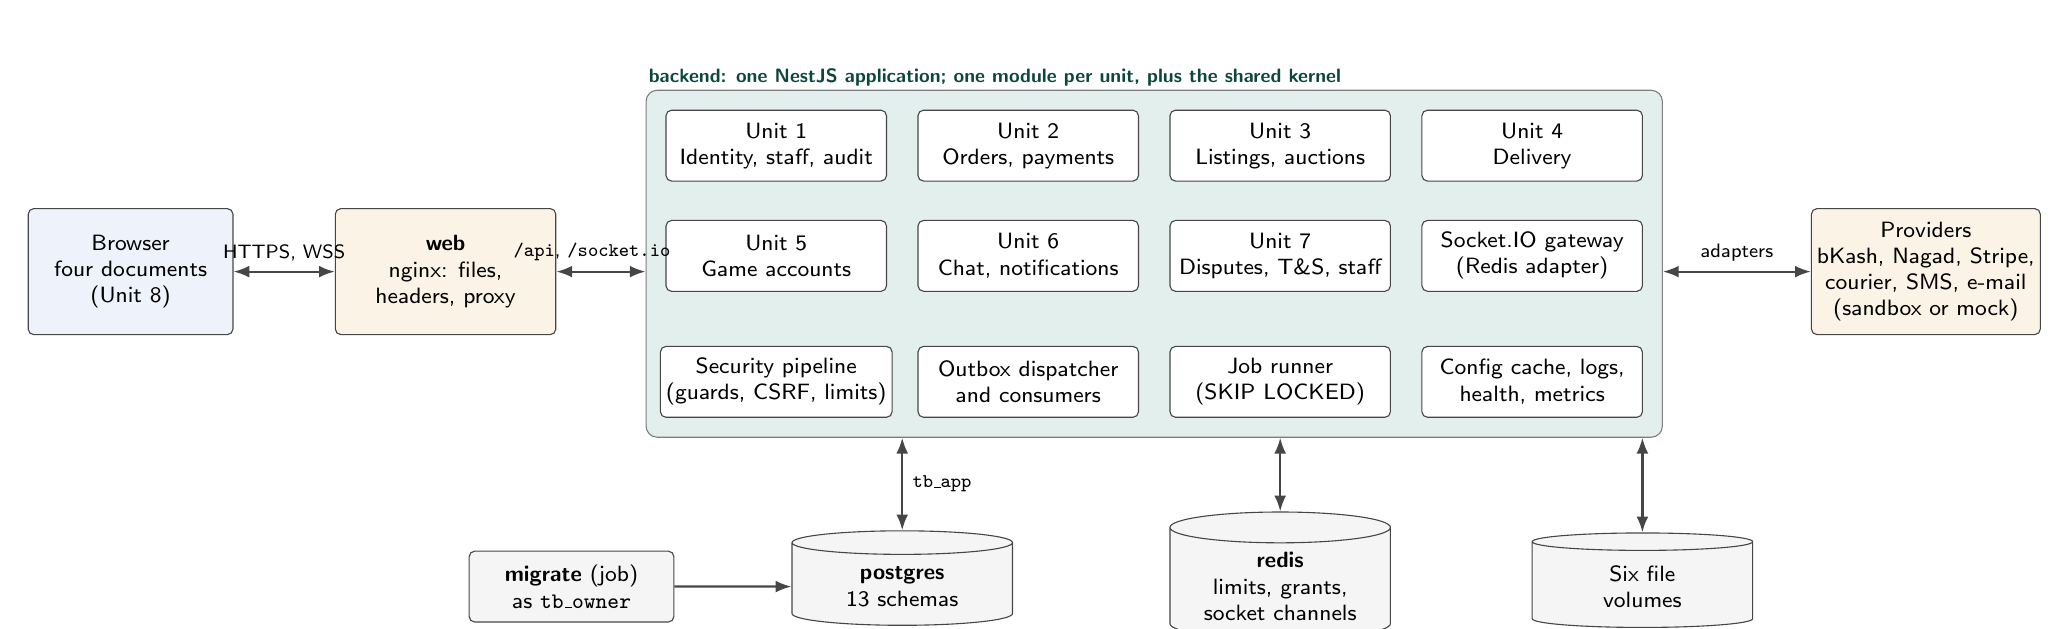
\begin{tikzpicture}[
  font=\sffamily\footnotesize,
  comp/.style={draw=edge, rounded corners=2pt, fill=white, minimum width=2.8cm, minimum height=0.9cm, align=center, inner sep=2pt},
  grp/.style={draw=edge!70, rounded corners=4pt, inner sep=7pt},
  lbl/.style={font=\sffamily\scriptsize\bfseries, text=headcolor, anchor=south west, inner sep=1pt},
  arr/.style={-{Latex[length=2mm]}, draw=edge, thick},
  store/.style={draw=edge, fill=boxd, cylinder, shape border rotate=90, aspect=0.18, minimum width=2.8cm, minimum height=1.2cm, align=center}
]
\node[comp, fill=boxb, minimum width=2.6cm, minimum height=1.6cm] (br) at (-3.6,3.0) {Browser\\four documents\\(Unit 8)};
\node[comp, fill=boxc, minimum width=2.8cm, minimum height=1.6cm] (web) at (0.4,3.0) {\textbf{web}\\nginx: files,\\headers, proxy};
\foreach \n/\x/\y/\t in {u1/4.6/4.6/{Unit 1\\Identity, staff, audit}, u2/7.8/4.6/{Unit 2\\Orders, payments}, u3/11.0/4.6/{Unit 3\\Listings, auctions},
  u4/14.2/4.6/{Unit 4\\Delivery}, u5/4.6/3.2/{Unit 5\\Game accounts}, u6/7.8/3.2/{Unit 6\\Chat, notifications}, u7/11.0/3.2/{Unit 7\\Disputes, T\&S, staff},
  k1/4.6/1.6/{Security pipeline\\(guards, CSRF, limits)}, k2/7.8/1.6/{Outbox dispatcher\\and consumers}, k3/11.0/1.6/{Job runner\\(SKIP LOCKED)}, k4/14.2/1.6/{Config cache, logs,\\health, metrics}}
  {\node[comp] (\n) at (\x,\y) {\t};}
\node[comp, minimum width=2.8cm] (gw) at (14.2,3.2) {Socket.IO gateway\\(Redis adapter)};
\begin{scope}[on background layer]\node[grp, fill=boxa, fit=(u1)(k4)(gw)] (be) {};\end{scope}
\node[lbl] at (be.north west) {\textbf{backend}: one NestJS application; one module per unit, plus the shared kernel};
\node[store] (pg) at (6.2,-1.0) {\textbf{postgres}\\13 schemas};
\node[store] (rd) at (11.0,-1.0) {\textbf{redis}\\limits, grants,\\socket channels};
\node[store] (fv) at (15.6,-1.0) {Six file\\volumes};
\node[comp, fill=boxd, minimum width=2.6cm] (mg) at (2.0,-1.0) {\textbf{migrate} (job)\\as \texttt{tb\_owner}};
\node[comp, fill=boxc, minimum width=2.8cm, minimum height=1.6cm] (pr) at (19.2,3.0) {Providers\\bKash, Nagad, Stripe,\\courier, SMS, e-mail\\(sandbox or mock)};
\draw[arr, {Latex[length=2mm]}-{Latex[length=2mm]}] (br) -- node[above, font=\sffamily\scriptsize]{HTTPS, WSS} (web);
\draw[arr, {Latex[length=2mm]}-{Latex[length=2mm]}] (web.east) -- node[above, font=\sffamily\scriptsize, pos=0.4]{\texttt{/api}, \texttt{/socket.io}} (be.west|-web.east);
\draw[arr, {Latex[length=2mm]}-{Latex[length=2mm]}] (pg.north|-be.south) -- node[right, font=\sffamily\scriptsize]{\texttt{tb\_app}} (pg.north);
\draw[arr, {Latex[length=2mm]}-{Latex[length=2mm]}] (rd.north|-be.south) -- (rd.north);
\draw[arr, {Latex[length=2mm]}-{Latex[length=2mm]}] (fv.north|-be.south) -- (fv.north);
\draw[arr] (mg) -- (pg);
\draw[arr, {Latex[length=2mm]}-{Latex[length=2mm]}] (be.east|-pr.west) -- node[above, font=\sffamily\scriptsize]{adapters} (pr.west);
\end{tikzpicture}}
\caption{The system. Four long-running containers (bold: web, backend, postgres, redis) and the one-shot migration job. Only the web container is reachable from outside; providers are reached only through the units' adapters.}
\label{fig:system}
\end{figure}

\begin{dtable}{@{}>{\raggedright\arraybackslash}p{2.6cm}>{\ttfamily\raggedright\arraybackslash}p{3.4cm}>{\raggedright\arraybackslash}p{9.2cm}@{}}
\toprule
\textbf{Module} & \textnormal{\textbf{Schemas}} & \textbf{Provides to other modules} \\ \midrule \endhead
Unit 1 & identity, audit & \texttt{IdentityQuery}, \texttt{IdentityCommands}, \texttt{ApprovalService}, \texttt{AuditService}, \texttt{RateLimiter}, \texttt{FileVault}, \texttt{IdentityCrypto}, \texttt{StaffQuery}; the security pipeline \\
Unit 2 & orders, payments & \texttt{OrdersPort}, \texttt{EscrowCommands}, \texttt{EscrowQuery}, \texttt{ProStatusQuery}; provider adapters \\
Unit 3 & listings, auctions & \texttt{ListingsPort}, \texttt{ListingsCommands}, \texttt{ListingsQueries}, \texttt{AuctionQuery} \\
Unit 4 & delivery & \texttt{DeliveryPort}, \texttt{DeliveryCommands}, \texttt{DeliveryQueries}; courier adapter \\
Unit 5 & game\_accounts & \texttt{GameAccountPort}, \texttt{GameAccountCommands}, \texttt{GameAccountQueries} \\
Unit 6 & chat, notify & \texttt{NotificationPort}, \texttt{Notifier}, \texttt{ChatCommands}, \texttt{BlockPort}; e-mail and SMS adapters \\
Unit 7 & disputes, trust, staff & \texttt{DisputeCommands}, \texttt{ReportCommands}, \texttt{SanctionPort}, \texttt{TrustQuery}, \texttt{ConfigPort} \\
\bottomrule
\end{dtable}
NestJS's module system enforces part of this: a module can inject only what another module exports, and each module exports only its ports. The ESLint import rules forbid a module from importing another module's internal files or entities (Section~\ref{sec:sdl}).

\subsection{How units talk}
\label{sec:talk}
The units use two kinds of contract, and the choice between them is a rule, not a matter of taste:
\begin{dtable}{@{}>{\raggedright\arraybackslash}p{2.8cm}>{\raggedright\arraybackslash}p{6.0cm}>{\raggedright\arraybackslash}p{6.4cm}@{}}
\toprule
\textbf{Contract} & \textbf{Use when} & \textbf{Guarantees} \\ \midrule \endhead
Port call in the caller's transaction (DC-13) & The other unit's change must happen together with this one, or not at all: freeze the escrow when a dispute opens; record the delivery event with the handover code. & Atomic. Locks taken in the order of DC-14 (listing, order, unit row, escrow, attempt), so two flows cannot deadlock each other. \\
Port query & A fact owned by another unit is needed now: the dispute window, a user's restrictions. & The owner's current answer; no copies of other units' data (DC-1). \\
Event through the outbox (DC-6) & Others should react, but this change does not depend on them: notices, rating eligibility, signals, hiding listings. & Written in the same transaction as the change, delivered at least once, consumed idempotently. A slow or failing consumer never blocks the publisher. \\
\bottomrule
\end{dtable}

\textbf{The outbox dispatcher.} Each unit has one outbox table (checked, Section~\ref{sec:checks}). One dispatcher in the shared kernel polls the seven outboxes every 5~seconds, with \texttt{SKIP LOCKED}. It hands each event to the consumers registered for its name in the same process, and marks it dispatched after all have returned. A consumer that fails is retried with growing delay; after 10 attempts the event is reported to the operators, and the other consumers are not affected, because each consumer records which events it has processed. Events also go to Socket.IO where a unit asked for a live message. Since everything runs in one process, no message broker is needed. A broker could be added later behind the dispatcher without changing any unit.

\textbf{Order of events.} Consumers may receive events out of order, for example \texttt{orders.\allowbreak escrow.\allowbreak released} before \texttt{orders.\allowbreak order.\allowbreak delivered} after a retry. Every unit designed its consumers for this: each consumer checks the state it changes. In Unit~2's words, ``a step or event that arrives twice, or for an order in the wrong state, is ignored and logged''; Unit~7's rating eligibility is keyed by the order, so a repeat changes nothing.

\subsection{One request, end to end}
A bid shows every layer:
\begin{enumerate}[nosep]
  \item The browser sends \texttt{POST /api/v1/auctions/\{id\}/bids} with its cookies, \texttt{X-CSRF-Token} and an \texttt{Idempotency-Key} (Unit~8).
  \item nginx forwards it to the backend on the internal network.
  \item The security pipeline (Unit~1) applies the rate limit, checks the token, the session, CSRF and the \texttt{Verified(bid)} policy, which asks \texttt{SanctionPort} (Unit~7) and \texttt{BlockPort} (Unit~6).
  \item \texttt{BidService} (Unit~3) runs \texttt{auctions.\allowbreak place\_\allowbreak bid} in one transaction. It writes the bid and, through the outbox, \texttt{auctions.\allowbreak bid.\allowbreak outbid}.
  \item After the commit, the gateway sends \texttt{auction.state} to the auction room through the Redis adapter, to every instance and every viewer.
  \item The dispatcher delivers \texttt{auctions.\allowbreak bid.\allowbreak outbid} to Unit~6, which creates the notice for the previous leader.
\end{enumerate}
The answer to the bidder is sent after step~4's commit, never earlier (NFR-REL-02). Steps~5 and~6 can be lost in a crash without harm: the auction state is in PostgreSQL, clients fetch it again on reconnection (Unit~8), and the outbox delivers the event after the restart (NFR-REL-01).

\subsection{Scaling and restarts}
No backend instance keeps state that another needs (NFR-SCL-02). Sessions are rows, rate limits and grants are Redis keys, live messages pass through the Socket.IO Redis adapter (NFR-SCL-01), and jobs claim rows with \texttt{SKIP LOCKED}. A second backend instance therefore needs only \texttt{docker compose up --scale backend=2} and a reload of nginx, which then forwards to both. Socket.IO's HTTP long-polling fallback would need sticky sessions; the client connects with the WebSocket transport only (I-65), so it does not arise. Redis is never the only copy of anything authoritative (IF-SW-09): losing it ends live connections, step-up grants and rate-limit counts, which are short-lived by design, and nothing else.
\section{The Combined Data Model}
\label{sec:data}

\subsection{Seven units, thirteen schemas}
The seven backend units' schemas load into one database, in unit order, followed by this unit's migration, which adds indexes only. The counts below are read from PostgreSQL's catalogue after loading.
\begin{dtable}{@{}c>{\raggedright\arraybackslash}p{2.6cm}rrrrrrr@{}}
\toprule
\textbf{Unit} & \textbf{Schema} & \textbf{Tables} & \textbf{Views} & \textbf{Functions} & \textbf{Triggers} & \textbf{Enums} & \textbf{Checks} & \textbf{Indexes} \\ \midrule \endhead
1 & \texttt{audit} & 1 & 0 & 2 & 2 & 1 & 1 & 5 \\
1 & \texttt{identity} & 20 & 0 & 2 & 2 & 13 & 65 & 54 \\
2 & \texttt{orders} & 5 & 0 & 1 & 2 & 10 & 34 & 15 \\
2 & \texttt{payments} & 13 & 1 & 3 & 5 & 9 & 45 & 35 \\
3 & \texttt{auctions} & 8 & 0 & 9 & 1 & 3 & 21 & 19 \\
3 & \texttt{listings} & 6 & 1 & 6 & 4 & 7 & 20 & 19 \\
4 & \texttt{delivery} & 14 & 0 & 20 & 9 & 12 & 46 & 32 \\
5 & \texttt{game\_accounts} & 10 & 0 & 19 & 8 & 5 & 33 & 22 \\
6 & \texttt{chat} & 7 & 0 & 9 & 4 & 2 & 11 & 19 \\
6 & \texttt{notify} & 8 & 0 & 8 & 1 & 5 & 12 & 16 \\
7 & \texttt{disputes} & 5 & 0 & 11 & 6 & 5 & 19 & 15 \\
7 & \texttt{staff} & 4 & 0 & 4 & 2 & 0 & 9 & 5 \\
7 & \texttt{trust} & 6 & 1 & 4 & 4 & 6 & 17 & 20 \\
\midrule
& \textbf{All} & 107 & 3 & 98 & 50 & 78 & 333 & 276 \\
\bottomrule
\end{dtable}
Units~1 and~2 keep most of their logic in the application services, so their schemas have few functions. Units~3 to~7 put their critical state changes into database functions, from bidding to dispute decisions, so the concurrency tests could exercise them directly. Every table has a primary key, every time is a \texttt{timestamptz}, and every amount of money is a \texttt{bigint} of poisha (checked below).

\textbf{References between units.} DC-5 allows a foreign key only to an earlier unit. Across all schemas, only six tables are referenced by another unit:
\begin{dtable}{@{}>{\raggedright\arraybackslash}p{2.0cm}cccccc@{}}
\toprule
& \multicolumn{4}{c}{\textbf{Unit 1:} \texttt{identity}} & \textbf{Unit 2} & \textbf{Unit 3} \\
\textbf{From} & \texttt{users} & \texttt{staff\_\allowbreak accounts} & \texttt{sessions} & \texttt{approvals} & \texttt{orders} & \texttt{listings} \\ \midrule \endhead
Unit 2 & 8 & 2 & & & --- & --- \\
Unit 3 & 9 & 2 & & & & --- \\
Unit 4 & 6 & 3 & & & 4 & 1 \\
Unit 5 & 4 & 1 & 3 & & 2 & 1 \\
Unit 6 & 10 & 2 & & & & 2 \\
Unit 7 & 13 & 10 & & 4 & 3 & \\
\bottomrule
\end{dtable}
Everything else between units goes through ports and events. Users, staff accounts, sessions and approvals are never deleted (Unit~1 erases a user's data in place), so these references can never block a deletion.

\subsection{The integration checks}
\label{sec:checks}
\texttt{09\_\allowbreak integration\_\allowbreak checks.\allowbreak sql} reads the catalogue of the combined database and checks every convention that spans units. It changes nothing, and the CI pipeline runs it after the unit tests (Section~\ref{sec:sdl}).
\begin{dtable}{@{}>{\raggedright\arraybackslash}p{6.4cm}>{\raggedright\arraybackslash}p{8.8cm}@{}}
\toprule
\textbf{Check} & \textbf{How} \\ \midrule \endhead
Every schema belongs to one unit; nothing in \texttt{public} & Schemas and objects outside the unit map, ignoring extension objects. \\
Convention DC-5 & Every foreign key's target unit is the same or earlier. \\
Convention DC-1 & Function bodies are searched for another unit's schema. A table of another unit may never appear. A function of another unit may be called only if it is \texttt{IMMUTABLE}, a pure calculation. The only such call is Unit~4's use of Unit~3's \texttt{listings.\allowbreak distance\_\allowbreak km}, a great-circle distance. \\
Triggers & A trigger runs its own unit's function, or the shared \texttt{identity.\allowbreak forbid\_\allowbreak change}. \\
Primary keys; types & Every table has a primary key; no \texttt{timestamp} without time zone, no float or money type; every money column is \texttt{bigint}. \\
SEC-INP-02 & No database function builds SQL at run time (no \texttt{EXECUTE}). \\
Convention DC-6 & One outbox per unit; each accepts only its own unit's event names; every event name a function writes has the form \texttt{<unit>.<entity>.<past>} of its own unit. \\
Convention DC-15 (new) & Indexes on foreign keys, below. \\
The application account & \texttt{tb\_app}: no superuser, role, database or RLS-bypass rights; owns nothing; no \texttt{TRUNCATE}, \texttt{TRIGGER} or \texttt{REFERENCES}; may not delete from any append-only table; may use every unit schema. \\
\bottomrule
\end{dtable}
All 21 checks pass on the combined schema. A check that has never failed proves little, so \texttt{09\_\allowbreak integration\_\allowbreak checks\_\allowbreak selftest.\allowbreak sh} builds a second database with one planted violation per check: an unknown schema, a table in \texttt{public}, a foreign key from Unit~1 to Unit~7, a function reading another unit's table, and so on. All 21 checks report FAIL there (Appendix~\ref{app:tests}).

\textbf{Convention DC-15.} The combined schema had 108 foreign keys without an index on their columns. An index is needed when the parent row can be deleted (otherwise each deletion scans the child table) or when a query or trigger looks rows up by the column. It is not needed for actor columns such as \texttt{decided\_by} that point to rows never deleted. \textbf{DC-15.} A foreign key has an index if the application may delete from its target table, or if any query, trigger or job looks rows up by it. The check found one case of the first kind: deleting a pending registration scanned \texttt{identity.\allowbreak otp\_\allowbreak challenges}. A review of every unit's queries found 23 of the second kind, for example the CP-33 evidence limit counting per dispute, the strike count per bidder in Unit~3, and the profile summary counting completed orders per user. \texttt{09\_\allowbreak integration.\allowbreak sql} adds these 24 indexes and changes nothing else.

\subsection{Migrations}
The design SQL files are the reference for the TypeORM migrations (NFR-MNT-04). One migration per unit file, applied in unit order and then \texttt{09\_\allowbreak integration.\allowbreak sql}, gives exactly the schema checked here. The migration job runs them as \texttt{tb\_owner}, a login role without superuser, role-creation or database-creation rights (SEC-INF-03). This works because the three extensions the units use (\texttt{citext}, \texttt{pgcrypto}, \texttt{pg\_trgm}) are trusted extensions, which the database owner may create. It was tested: all eight migrations ran as \texttt{tb\_owner}, and \texttt{tb\_app} could read and write data but was refused ten kinds of schema change, including deletes from an append-only table (Appendix~\ref{app:tests}). Schema synchronisation by the ORM is turned off everywhere except a developer's scratch database (SEC-INF-05).

% ------------------------------------------------------------------
\section{Catalogues}
\label{sec:catalogues}

\subsection{Events}
\label{sec:events}
\texttt{check\_\allowbreak documents.\allowbreak py} reads the events tables of all units, expands their abbreviations (\texttt{.refunded} after \texttt{orders.\allowbreak escrow.\allowbreak released}), adds the event names the database functions write, and matches publishers with consumers. Of the 68\unskip{} events published, the table lists which units consume each. Unit~6 creates notices from almost all of them; its own table lists them by family.
{\small
\begin{longtable}{@{}>{\raggedright\arraybackslash}p{8.0cm}>{\centering\arraybackslash}p{1.8cm}>{\raggedright\arraybackslash}p{5.0cm}@{}}
\toprule
\textbf{Event} & \textbf{Publisher} & \textbf{Consumed by units} \\ \midrule \endhead
\texttt{identity.\allowbreak account.\allowbreak closed} & 1 & 4, 7 \\
\texttt{identity.\allowbreak account.\allowbreak reinstated} & 1 & 3, 6 \\
\texttt{identity.\allowbreak account.\allowbreak suspended} & 1 & 3, 6 \\
\texttt{identity.\allowbreak contact.\allowbreak changed} & 1 & 6 \\
\texttt{identity.\allowbreak email.\allowbreak verified} & 1 & none listed \\
\texttt{identity.\allowbreak kyc.\allowbreak rejected} & 1 & 6 \\
\texttt{identity.\allowbreak kyc.\allowbreak revoked} & 1 & 3 \\
\texttt{identity.\allowbreak kyc.\allowbreak submitted} & 1 & none listed \\
\texttt{identity.\allowbreak kyc.\allowbreak verified} & 1 & 3, 6 \\
\texttt{identity.\allowbreak mfa.\allowbreak disabled} & 1 & 6 \\
\texttt{identity.\allowbreak mfa.\allowbreak enabled} & 1 & 6 \\
\texttt{identity.\allowbreak password.\allowbreak changed} & 1 & 6 \\
\texttt{identity.\allowbreak session.\allowbreak reuse\_\allowbreak detected} & 1 & none listed \\
\texttt{identity.\allowbreak signin.\allowbreak new\_\allowbreak device} & 1 & 6 \\
\texttt{identity.\allowbreak user.\allowbreak registered} & 1 & none listed \\
\texttt{orders.\allowbreak escrow.\allowbreak frozen} & 2 & 6 \\
\texttt{orders.\allowbreak escrow.\allowbreak partially\_\allowbreak refunded} & 2 & 5, 6, 7 \\
\texttt{orders.\allowbreak escrow.\allowbreak refunded} & 2 & 4, 5, 6, 7 \\
\texttt{orders.\allowbreak escrow.\allowbreak released} & 2 & 5, 6, 7 \\
\texttt{orders.\allowbreak order.\allowbreak cancelled} & 2 & 3 \\
\texttt{orders.\allowbreak order.\allowbreak cancelled\_\allowbreak by\_\allowbreak seller} & 2 & 7 \\
\texttt{orders.\allowbreak order.\allowbreak created} & 2 & 6 \\
\texttt{orders.\allowbreak order.\allowbreak delivered} & 2 & 6 \\
\texttt{orders.\allowbreak order.\allowbreak paid} & 2 & 3, 4, 5, 6 \\
\texttt{orders.\allowbreak order.\allowbreak payment\_\allowbreak expired} & 2 & 3 \\
\texttt{payments.\allowbreak featured.\allowbreak ended} & 2 & 3 \\
\texttt{payments.\allowbreak featured.\allowbreak started} & 2 & 3 \\
\texttt{payments.\allowbreak payout.\allowbreak failed} & 2 & 6 \\
\texttt{payments.\allowbreak payout\_\allowbreak account.\allowbreak changed} & 2 & 6 \\
\texttt{payments.\allowbreak refund.\allowbreak manual\_\allowbreak required} & 2 & 6 \\
\texttt{payments.\allowbreak subscription.\allowbreak changed} & 2 & 3 \\
\texttt{auctions.\allowbreak auction.\allowbreak awarded} & 3 & 6 \\
\texttt{auctions.\allowbreak auction.\allowbreak cancelled} & 3 & none listed \\
\texttt{auctions.\allowbreak auction.\allowbreak unsold} & 3 & 6 \\
\texttt{auctions.\allowbreak bid.\allowbreak outbid} & 3 & 6 \\
\texttt{auctions.\allowbreak bidder.\allowbreak restricted} & 3 & none listed \\
\texttt{auctions.\allowbreak flag.\allowbreak raised} & 3 & 7 \\
\texttt{auctions.\allowbreak offer.\allowbreak expired} & 3 & 6 \\
\texttt{auctions.\allowbreak offer.\allowbreak made} & 3 & 6 \\
\texttt{listings.\allowbreak listing.\allowbreak cancelled} & 3 & 5 \\
\texttt{listings.\allowbreak listing.\allowbreak ended\_\allowbreak unsold} & 3 & 5 \\
\texttt{listings.\allowbreak listing.\allowbreak published} & 3 & 6 \\
\texttt{listings.\allowbreak listing.\allowbreak relisting\_\allowbreak flagged} & 3 & 7 \\
\texttt{listings.\allowbreak listing.\allowbreak removed} & 3 & 5, 6 \\
\texttt{listings.\allowbreak listing.\allowbreak sold} & 3 & none listed \\
\texttt{delivery.\allowbreak handover.\allowbreak completed} & 4 & 6 \\
\texttt{delivery.\allowbreak handover.\allowbreak locked} & 4 & 6 \\
\texttt{delivery.\allowbreak issue.\allowbreak opened} & 4 & 7 \\
\texttt{delivery.\allowbreak meetup.\allowbreak agreed} & 4 & 6 \\
\texttt{delivery.\allowbreak meetup.\allowbreak proposed} & 4 & 6 \\
\texttt{delivery.\allowbreak return.\allowbreak delivered} & 4 & 7 \\
\texttt{delivery.\allowbreak shipment.\allowbreak status\_\allowbreak changed} & 4 & 6 \\
\texttt{game\_\allowbreak accounts.\allowbreak credentials.\allowbreak delivered} & 5 & 6 \\
\texttt{game\_\allowbreak accounts.\allowbreak credentials.\allowbreak reported\_\allowbreak invalid} & 5 & 6 \\
\texttt{game\_\allowbreak accounts.\allowbreak credentials.\allowbreak requested} & 5 & 6 \\
\texttt{game\_\allowbreak accounts.\allowbreak ownership.\allowbreak approved} & 5 & 6 \\
\texttt{game\_\allowbreak accounts.\allowbreak ownership.\allowbreak rejected} & 5 & 6 \\
\texttt{game\_\allowbreak accounts.\allowbreak rekey.\allowbreak overdue} & 5 & 6 \\
\texttt{game\_\allowbreak accounts.\allowbreak rekey.\allowbreak requested} & 5 & 6 \\
\texttt{game\_\allowbreak accounts.\allowbreak takeover.\allowbreak completed} & 5 & 6 \\
\texttt{chat.\allowbreak message.\allowbreak flagged} & 6 & 7 \\
\texttt{disputes.\allowbreak dispute.\allowbreak decided} & 7 & none listed \\
\texttt{disputes.\allowbreak dispute.\allowbreak opened} & 7 & none listed \\
\texttt{disputes.\allowbreak dispute.\allowbreak withdrawn} & 7 & none listed \\
\texttt{staff.\allowbreak config.\allowbreak published} & 7 & none listed \\
\texttt{trust.\allowbreak report.\allowbreak resolved} & 7 & none listed \\
\texttt{trust.\allowbreak sanction.\allowbreak applied} & 7 & none listed \\
\texttt{trust.\allowbreak sanction.\allowbreak lifted} & 7 & none listed \\
\bottomrule
\end{longtable}
}

\subsection{Events added by integration}
The check found four events that a unit consumes, or a database function writes, but that no publisher's events table lists. Each was asked for in an integration note or described only in a unit's text; this catalogue makes them part of the contract.
\begin{dtable}{@{}>{\raggedright\arraybackslash}p{5.6cm}>{\raggedright\arraybackslash}p{1.6cm}>{\raggedright\arraybackslash}p{8.0cm}@{}}
\toprule
\textbf{Event} & \textbf{Publisher} & \textbf{Origin} \\ \midrule \endhead
\texttt{listings.\allowbreak listing.\allowbreak cancelled} & Unit 3 & I-30: Unit~5 releases a player-ID claim when a listing is cancelled (FR-LST-08). \\
\texttt{listings.\allowbreak listing.\allowbreak relisting\_\allowbreak flagged} & Unit 3 & I-45: Unit~7's flagged-activity queue (FR-TNS-02). \\
\texttt{delivery.\allowbreak issue.\allowbreak opened} & Unit 4 & I-46: Unit~7's flagged-activity queue. \\
\texttt{chat.\allowbreak message.\allowbreak flagged} & Unit 6 & Written by \texttt{chat.post}; described in Unit~6's detection section, not in an events table. \\
\bottomrule
\end{dtable}
With these, every consumed event has a publisher, and every event the database writes is listed (Section~\ref{sec:doccheck}).

\subsection{Ports}
\label{sec:ports}
Each unit declared the ports it provides as TypeScript interfaces, and the ports it needs with the unit that provides them. The check matches the two sides. Four ports were named by later units but never declared by their owner: Unit~1's \texttt{FileVault} and \texttt{IdentityCrypto} appear only as components, \texttt{StaffQuery} was first asked for by Unit~7, and \texttt{ListingsQueries} by Unit~4 (I-23). Their interfaces, from what the units say about them:
\begin{lstlisting}[language=Java,morekeywords={interface,type,Promise,string,boolean,number,bigint}]
interface FileVault {                  // Unit 1: protected files of every purpose
  store(f: { purpose: FilePurpose; ownerId: string; bytes: Uint8Array }, tx?: EntityManager)
    : Promise<{ key: string; sha256: string; mime: string; size: number }>;  // type from content (SEC-INP-04),
                                                                            // re-encoded, metadata removed (SEC-DAT-08)
  signedLink(key: string, viewer: Principal, reason?: string): Promise<string>;  // CP-31; staff views audited
  erase(key: string): Promise<void>;                                            // data key destroyed
}
type FilePurpose = 'kyc' | 'ownership_proof' | 'dispute_evidence' | 'chat_image' | 'data_export';
                                       // one volume each; KYC, proofs, evidence and exports encrypted per file
interface IdentityCrypto {             // Unit 1: field encryption for other units (Unit 4 addresses)
  encrypt(plain: string, context: string): Promise<Uint8Array>;  // AES-256-GCM, FIELD_KEY_V{n}; context as AD
  decrypt(sealed: Uint8Array, context: string): Promise<string>;
}
interface StaffQuery {                 // Unit 1: the conflict check of FR-OPS-06, at every claim (Unit 7)
  assertNoConflict(staffId: string, userIds: string[]): Promise<void>;  // same number, e-mail or NID, or declared
}
interface ListingsQueries {            // Unit 3
  fulfilmentFacts(listingId: string): Promise<{ options: Fulfilment[]; sizeClass: SizeClass;
                                              district: string; approxLat: number; approxLng: number }>; // Unit 4
  threadFacts(listingId: string): Promise<{ sellerId: string; title: string; status: ListingStatus }>;  // Unit 6
}
\end{lstlisting}
\begin{dtable}{@{}>{\raggedright\arraybackslash}p{5.0cm}>{\centering\arraybackslash}p{2.0cm}>{\raggedright\arraybackslash}p{8.2cm}@{}}
\toprule
\textbf{Port} & \textbf{Provider} & \textbf{Required by units} \\ \midrule \endhead
\texttt{ApprovalService} & 1 & 7 \\
\texttt{AuditService} & 1 & 4, 5, 7 \\
\texttt{FileVault} & 1 & 5, 6, 7 \\
\texttt{IdentityCommands} & 1 & 7 \\
\texttt{IdentityCrypto} & 1 & 4 \\
\texttt{IdentityQuery} & 1 & 4, 5, 6 \\
\texttt{RateLimiter} & 1 & 4 \\
\texttt{StaffQuery} & 1 & 7 \\
\texttt{EscrowCommands} & 2 & 4, 5, 7 \\
\texttt{EscrowQuery} & 2 & 7 \\
\texttt{OrdersPort} & 2 & 4, 5, 7 \\
\texttt{PaymentProvider} & 2 & --- \\
\texttt{PayoutProvider} & 2 & --- \\
\texttt{ProStatusQuery} & 2 & --- \\
\texttt{AuctionQuery} & 3 & 6 \\
\texttt{ListingsCommands} & 3 & 5, 7 \\
\texttt{ListingsPort} & 3 & --- \\
\texttt{ListingsQueries} & 3 & 4, 6 \\
\texttt{CourierPort} & 4 & --- \\
\texttt{DeliveryCommands} & 4 & 7 \\
\texttt{DeliveryPort} & 4 & --- \\
\texttt{DeliveryQueries} & 4 & 7 \\
\texttt{GameAccountCommands} & 5 & --- \\
\texttt{GameAccountPort} & 5 & --- \\
\texttt{GameAccountQueries} & 5 & 7 \\
\texttt{BlockPort} & 6 & --- \\
\texttt{ChatCommands} & 6 & 7 \\
\texttt{NotificationPort} & 6 & --- \\
\texttt{Notifier} & 6 & 7 \\
\texttt{ConfigPort} & 7 & --- \\
\texttt{DisputeCommands} & 7 & 5 \\
\texttt{ReportCommands} & 7 & 6 \\
\texttt{SanctionPort} & 7 & --- \\
\texttt{TrustQuery} & 7 & --- \\
\bottomrule
\end{dtable}

\subsection{Redis keys}
Redis holds nothing authoritative (IF-SW-09). Its keys belong to the shared kernel or Unit~1, so there is no collision between units:
\begin{dtable}{@{}>{\ttfamily\raggedright\arraybackslash}p{4.4cm}>{\raggedright\arraybackslash}p{2.4cm}>{\raggedright\arraybackslash}p{8.4cm}@{}}
\toprule
\textnormal{\textbf{Key or channel}} & \textbf{Owner} & \textbf{Use; lost on a Redis restart, then} \\ \midrule \endhead
rl:\{rule\}:\{subject\} & Unit 1 & Rate-limit counters for every unit's limits (CP-04, CP-05, CP-35); counting restarts. \\
signin:fail:\{account\} & Unit 1 & Sign-in failure delay; restarts at zero. \\
mfa:ticket:\{hash\} & Unit 1 & MFA step of sign-in (5 minutes); the user signs in again. \\
stepup:\{sid\}:\{action\} & Unit 1 & Single-use step-up grants; the user enters a new OTP. \\
socket.io\#/\# \dots & Gateway & Socket.IO adapter channels for the rooms \texttt{sid:}, \texttt{user:} and \texttt{auction:}; clients reconnect and resync (IF-COM-02). \\
\bottomrule
\end{dtable}
Redis runs without persistence and with \texttt{noeviction} (DV-65): when memory is full, a write fails visibly instead of a counter or grant silently disappearing.

\subsection{Scheduled jobs}
\label{sec:jobs}
Every unit's jobs run in every backend instance. Each job selects its due rows with \texttt{FOR UPDATE SKIP LOCKED}, re-checks the state inside its transaction, and acts on the recorded due time. Several instances can therefore run the same job without a leader, and a job that was down catches up exactly once (NFR-REL-03). The job runner in the shared kernel starts each loop at its interval with 10\% random spread (DV-67), and records each run's duration and outcome as metrics.
\begin{dtable}{@{}>{\raggedright\arraybackslash}p{1.1cm}>{\raggedright\arraybackslash}p{11.6cm}>{\raggedright\arraybackslash}p{2.3cm}@{}}
\toprule
\textbf{Unit} & \textbf{Jobs} & \textbf{Fastest} \\ \midrule \endhead
1 & Erasure after closure (FR-PRV-04); rejected KYC images after 30 days; expiry of four-eyes proposals (DV-5); audit hash-chain verification (SEC-LOG-02). & daily \\
2 & Payment expiry; fulfilment deadline; auto-release; refund and payout workers; reconciliation (CP-46); stalled delivery; cancellation lapse; monetization. & 30 s \\
3 & Auction closer (after the close grace DV-17); expiry of second-chance offers. & a few seconds \\
4 & Courier booking; status reconciliation; proposal lapse; address erasure; provider-event retention. & 1 min \\
5 & Takeover-window end; overdue re-key; proof expiry. & 1 min \\
6 & E-mail and SMS delivery; reminders and ending-soon notices; chat and notification retention. & continuous \\
7 & Seller-response deadlines; decision targets; signal aggregation; data exports. & 5 min \\
Kernel & The outbox dispatcher for all seven outboxes. It replaces the dispatchers that Units~2 and~7 listed among their jobs, so there is one implementation. & 5 s \\
\bottomrule
\end{dtable}
\section{Deployment}
\label{sec:deploy}

\subsection{Containers}
The reference Compose files are in \texttt{docs/design/deploy/} and go to the repository root. They replace the current \texttt{docker-compose.\allowbreak yml}, which runs development servers, publishes the database and Redis ports to the host, and sets no Redis password.
\begin{dtable}{@{}>{\ttfamily\raggedright\arraybackslash}p{1.8cm}>{\raggedright\arraybackslash}p{3.7cm}>{\raggedright\arraybackslash}p{9.7cm}@{}}
\toprule
\textnormal{\textbf{Service}} & \textbf{Image} & \textbf{Runs as, and why so} \\ \midrule \endhead
postgres & \texttt{postgres:15-alpine} & IF-SW-09. SCRAM passwords; the first start creates \texttt{tb\_owner}, \texttt{tb\_app} and the database (\texttt{postgres/init/01\_\allowbreak roles.\allowbreak sh}). Internal network only. \\
redis & \texttt{redis:7-alpine} & Password required; no persistence; \texttt{noeviction} (DV-65); read-only root; internal network only. \\
migrate & the backend image & One-shot job: applies the migrations as \texttt{tb\_owner} and exits. The backend starts only after it succeeded. \\
backend & \texttt{node:20-alpine}, two stages & User 10001; read-only root, \texttt{/tmp} in memory; all capabilities dropped; six file volumes; on both networks; port 3000 not published. \\
web & \texttt{nginx-\allowbreak unprivileged:\allowbreak 1.27-alpine}, two stages & User 101; Unit~8's tested nginx configuration and headers; the only published port. \\
\bottomrule
\end{dtable}
NFR-MNT-01 asks for four containers. These are the four long-running ones. The migration job runs once and exits before the backend starts, so the backend never holds the owner's password. Running migrations inside the backend container would need that password there, which SEC-INF-03 is meant to prevent. An SRS clarification states this reading (I-66).

\textbf{Networks} (SEC-INF-02). \texttt{data} is an internal network: PostgreSQL and Redis are on it alone, unreachable from the host or the outside, and the web container is not on it. \texttt{edge} connects the web container and the backend. Only the web container's port 8080 is published.

\textbf{Files.} Each file purpose has its own named volume, mounted only in the backend: KYC images, listing photos, ownership proofs, chat images, dispute evidence and data exports. The image creates the mount points owned by the backend's user with mode 0700, so new volumes inherit that ownership.

\subsection{Starting it}
\label{sec:start}
\textbf{Development} (NFR-MNT-08): \texttt{docker compose up --build} on any machine with Docker, with no other step. Every secret has a development value that is at least 32 bytes long and starts with \texttt{dev-only-}. Payments, couriers, SMS and e-mail run in mock or log mode (C-2, C-3). Verification links and OTPs appear in the backend's log in development only.

\textbf{Production:} \texttt{docker compose -f docker-compose.\allowbreak yml -f docker-compose.\allowbreak prod.\allowbreak yml --env-file prod.\allowbreak env up -d}. The override replaces every development value with a required variable, so Compose refuses to start while any secret is missing and names it. It sets \texttt{NODE\_\allowbreak ENV=production} (SEC-INF-05) and binds the web port to the loopback interface, behind the TLS front: a reverse proxy on the host or the hosting provider's load balancer, which terminates HTTPS, sets HSTS and forwards to port 8080 (SEC-DAT-01). \texttt{prod.\allowbreak env.\allowbreak example} lists every value; the test checks that it lists all that the override requires. The backend also refuses to start in production if any secret still starts with \texttt{dev-only-} (I-59). Development, test and production use different values, and production data is never copied to the others (SEC-INF-04).

\textbf{Order of start.} \texttt{postgres} and \texttt{redis} become healthy; \texttt{migrate} applies the migrations and exits successfully; \texttt{backend} starts and becomes ready; \texttt{web} starts. A failed migration stops the whole start, so an application never runs on a schema it does not expect.

\textbf{Health} (NFR-OBS-01, DV-61). \texttt{GET /api/v1/health/live} answers if the process runs. \texttt{GET /api/v1/health/ready} also checks PostgreSQL with \texttt{SELECT 1} and Redis with \texttt{PING}, each within 2~seconds. Compose uses \texttt{ready} for the backend's health check and nginx's \texttt{/healthz} for the web container's.

\textbf{Shutdown} (DV-66). On \texttt{SIGTERM}, the backend stops accepting requests and jobs, finishes the requests in progress, and closes live connections. Clients reconnect to another instance or after the restart, then resync. Compose allows 30~seconds before it forces the stop.

\subsection{Secrets and settings}
\begin{dtable}{@{}>{\raggedright\arraybackslash}p{2.0cm}>{\raggedright\arraybackslash}p{6.4cm}>{\raggedright\arraybackslash}p{6.8cm}@{}}
\toprule
\textbf{Unit} & \textbf{Secrets} & \textbf{Settings} \\ \midrule \endhead
Unit 9 & \texttt{POSTGRES\_\allowbreak PASSWORD} (first start only), \texttt{TB\_\allowbreak OWNER\_\allowbreak PASSWORD}, \texttt{TB\_\allowbreak APP\_\allowbreak PASSWORD}, \texttt{REDIS\_\allowbreak PASSWORD} & \texttt{PUBLIC\_\allowbreak ORIGIN}, \texttt{TB\_VERSION}, \texttt{TB\_\allowbreak HTTP\_\allowbreak PORT} \\
Unit 1 & \texttt{JWT\_KEY\_V1}, \texttt{FIELD\_\allowbreak KEY\_\allowbreak V1}, \texttt{BIDX\_KEY}, \texttt{KYC\_KEK\_V1}, \texttt{CSRF\_KEY}, \texttt{LINK\_KEY}, \texttt{OTP\_PEPPER} & --- \\
Unit 2 & \texttt{CALLBACK\_\allowbreak STATE\_\allowbreak KEY}; Stripe, bKash and Nagad credentials & \texttt{PAYMENT\_MODE} \\
Unit 4 & \texttt{HANDOVER\_KEY}; courier key and webhook secret & \texttt{COURIER\_MODE} \\
Unit 6 & \texttt{SMTP\_URL}, \texttt{SMS\_API\_KEY} & \texttt{SMS\_MODE}, \texttt{EMAIL\_MODE} \\
Unit 8 & --- & \texttt{VITE\_\allowbreak PAYMENT\_\allowbreak HOSTS} (build time) \\
\bottomrule
\end{dtable}
Each secret is at least 32 bytes and is read once at start-up, never logged (SEC-DAT-05). Rotation follows each owning unit's rules (Unit~1, Section~7). The business parameters CP-01 to CP-47 are not settings at all: they live in Unit~7's versioned store (NFR-MNT-06).

\subsection{Backups and restore}
\label{sec:backup}
\begin{itemize}[nosep]
  \item \textbf{Database} (NFR-REL-05). Nightly at 02:30 Dhaka time, \texttt{pg\_dump} in custom format, kept for 14 days and as 8 weekly copies (DV-64). In production, continuous WAL archiving as well, for a recovery point of 15~minutes and a recovery time of 4~hours. Roles are not part of a dump: the init script recreates them before a restore.
  \item \textbf{Files.} The six volumes are copied nightly. KYC images, proofs, evidence and exports are encrypted per file, and their keys are not on the volumes, so a stolen backup of the files reveals nothing (Unit~1). The keys are backed up separately, offline.
  \item \textbf{Restore test} (NFR-REL-05, before each release). \texttt{09\_\allowbreak backup\_\allowbreak restore\_\allowbreak test.\allowbreak sh} dumps and restores the database in five rounds: the seeded schema, then the data written by each of the Unit~4 to~7 concurrency scripts. It checks that every table has the same rows afterwards and that the integration checks pass. It also runs every unit's test script on the restored seeded schema. All five rounds passed (Appendix~\ref{app:tests}).
\end{itemize}

% ------------------------------------------------------------------
\section{Operation}
\label{sec:ops}

\subsection{Logs and metrics}
\begin{itemize}[nosep]
  \item \textbf{Logs} (NFR-OBS-02, DV-62). One JSON object per line to standard output, with time (UTC), level, module (the unit), message and the request's correlation id. Docker rotates them (5 files of 50~MB per container). Before writing, the logger removes the fields SEC-DAT-07 forbids, by key: \texttt{password}, \texttt{otp}, \texttt{token}, \texttt{cookie}, \texttt{authorization}, \texttt{nid}, \texttt{accountNumber}, \texttt{ciphertext}, \texttt{credentials}. It masks phone numbers and e-mail addresses to their last characters, and it never logs request or response bodies.
  \item \textbf{Metrics} (NFR-OBS-03, DV-63). Prometheus format on port 9464 inside the \texttt{edge} network, which nginx does not forward, so metrics are not public. They cover request rate, errors and latency by route; open WebSocket connections; outbox depth and age per unit; job runs, durations and failures per job; and the provider adapters' errors.
  \item \textbf{Alerts} (SEC-LOG-05). The events SEC-LOG-05 names are counted as metrics, with these thresholds: failed sign-ins above 5 times the hourly average; OTP sends above 3 times; more than 20 KYC image views by one staff member in an hour; any break in the audit hash chain; repeated webhook signature failures; and any rejected escrow transition. An outbox older than 5~minutes and a job failing three times in a row are alerts too.
\end{itemize}

\subsection{Retention}
\label{sec:retention}
NFR-CMP-01 asks that the SRS retention schedule be followed. Matching each row with the job that deletes the data found three without one:
\begin{dtable}{@{}>{\raggedright\arraybackslash}p{4.4cm}>{\raggedright\arraybackslash}p{4.4cm}>{\raggedright\arraybackslash}p{6.4cm}@{}}
\toprule
\textbf{Data (SRS schedule)} & \textbf{Kept} & \textbf{Done by} \\ \midrule \endhead
KYC images, NID number & 30 days after closure or rejection & Unit~1 erasure job \\
NID blind index on the blacklist & while the entry exists & Unit~1 \\
Game-account ciphertext & until the order is terminal & Unit~5 \texttt{finish} \\
Credential-access log & 2 years after the order closes & \textbf{missing}: Unit~5 job (I-63) \\
Settlement records, refunds, payouts & 6 years & \textbf{missing}: Unit~2 job, needed from year six (I-63) \\
Audit and security logs & at least CP-40 & kept: the hash chain must stay whole (Unit~1) \\
Chat messages & 1 year after the last message, unless held & Unit~6 \texttt{purge\_due} \\
Dispute case files & 2 years after the decision & \textbf{missing}: Unit~7 job for statements and evidence files (I-63) \\
Account data after closure & within CP-41 & Unit~1 erasure job \\
Design values: shipments, notices, provider events, ownership screenshots & DV-30, DV-42, CP-32, DV-39 & Units~4 and~6; Unit~5's screenshots also need their job (I-63) \\
\bottomrule
\end{dtable}

\subsection{Incidents and vulnerabilities}
\begin{itemize}[nosep]
  \item \textbf{Vulnerabilities} (SEC-IRM-01). Findings from Dependabot, \texttt{npm audit}, image scans and CodeQL are fixed within CP-42: 7 days for critical, 30 days for high.
  \item \textbf{Security contact} (SEC-IRM-02). \texttt{/.\allowbreak well-known/security.\allowbreak txt} gives the same contacts as the repository's \texttt{SECURITY.md} (GitHub private vulnerability reporting, and the team's address), the preferred languages (English, Bangla) and the expiry date that RFC~9116 requires; the web image includes it.
  \item \textbf{Incident procedure} (SEC-IRM-03). Roles: one team member leads, one investigates, one communicates. To contain an incident, use the emergency switches of SEC-IRM-04 (Unit~7: stop new orders, stop payouts, turn the game-account feature off), end all sessions, and rotate the affected keys. To preserve evidence, the audit log is append-only and hash-chained; snapshot the database and copy the logs before any change. For a personal-data breach, notify the authority and the affected users as the PDPO requires (NFR-CMP-01). The procedure is added to \texttt{SECURITY.md}, next to the reporting contacts it already has, and is rehearsed once before the demonstration.
\end{itemize}
\section{Secure Development}
\label{sec:sdl}

\subsection{The pipeline}
The reference workflows are in \texttt{docs/design/deploy/github/} and go to \texttt{.github/}. actionlint reports no problems in them. Every action is pinned to a commit, not a tag, so a changed tag cannot change the pipeline.
\begin{dtable}{@{}>{\raggedright\arraybackslash}p{3.0cm}>{\raggedright\arraybackslash}p{8.6cm}>{\raggedright\arraybackslash}p{3.6cm}@{}}
\toprule
\textbf{Job} & \textbf{What it runs} & \textbf{Requirements} \\ \midrule \endhead
lint-and-unit & For backend and frontend: \texttt{npm ci}, ESLint, \texttt{npm audit --audit-level=high}, unit tests with coverage thresholds of 70\% for the auction, order, payment, escrow, delivery and game-account modules. & NFR-MNT-03, NFR-MNT-07, SEC-SDL-02, SEC-SDL-04 \\
database & PostgreSQL 15 service: every schema and test script, the integration checks; the concurrency suites, each on a fresh database; the negative control; backup and restore. & NFR-MNT-02, SEC-SDL-02, NFR-REL-05 \\
reference-browser & Unit~5's \texttt{sealed.js} and Unit~8's web modules in Chromium; the web container's headers in nginx. & SEC-GEN-03 \\
documents & \texttt{check\_\allowbreak documents.\allowbreak py} over the SRS and the nine units; the Compose test. & Section~\ref{sec:doccheck} \\
images & Builds the two images; Trivy fails on a fixable critical or high finding; an SPDX SBOM of the backend. & SEC-SDL-06, SEC-SDL-07 \\
CodeQL & JavaScript and TypeScript with the security-extended queries, on every pull request and weekly; a new high finding blocks the merge. & SEC-SDL-03, SEC-INP-02 \\
ZAP baseline & On demand, against the Compose system of the release candidate; findings triaged before the demonstration. & SEC-SDL-08 \\
\bottomrule
\end{dtable}
\textbf{Repository settings} (not files, set once by the owner): \texttt{main} protected; changes only by pull request with CI passing and one approving review by someone other than the author; a security review, by a reviewer who did not write the change, for changes under \texttt{auth}, \texttt{payments}, \texttt{escrow}, \texttt{game-accounts} and the security pipeline, enforced with \texttt{CODEOWNERS} (SEC-SDL-01). Secret scanning with push protection is on; a secret found in history is rotated, not just deleted (SEC-SDL-05). Dependabot updates npm packages, actions and base images weekly (SEC-SDL-04).

\textbf{ESLint rules that carry design decisions:} \texttt{no-restricted-imports} keeps each module to its own files and the other modules' ports (DC-1, Section~\ref{sec:system}); \texttt{react/no-danger} and a ban on \texttt{innerHTML} (Unit~8); \texttt{no-restricted-syntax} forbids SQL built with template strings or \texttt{+} in calls to \texttt{query} (SEC-INP-02, backed by CodeQL's injection queries); \texttt{localStorage} only in the modules Unit~8 allows.

\subsection{Threat model}
\label{sec:threats}
SEC-GEN-02 asks for a threat model of each area before it is built. Units~1, 4, 5 and~7 have a table of threats and controls; Units~2, 3, 6 and~8 describe their controls in their security sections. The table gathers the main threats of every area, grouped by STRIDE, with the control and where it is designed:
{\small
\begin{longtable}{@{}>{\raggedright\arraybackslash}p{2.0cm}>{\raggedright\arraybackslash}p{5.2cm}>{\raggedright\arraybackslash}p{6.0cm}>{\raggedright\arraybackslash}p{1.8cm}@{}}
\toprule
\textbf{Area} & \textbf{Threat (STRIDE)} & \textbf{Control} & \textbf{Where} \\ \midrule \endhead
Identity & Account takeover by password guessing (S) & Argon2id, growing delay, MFA, new-device alerts & U1 \S7 \\
 & A stolen refresh token reused (S) & Rotation with reuse detection; whole session family ended & U1 \S6 \\
 & Insider browsing KYC images (I) & Claim, reason per image, audit, volume alert & U1 \S7 \\
Payments & Forged payment confirmation (T) & Server-to-server confirmation only; signature or verification query; amount from the server & U2 \S6 \\
 & The same webhook twice (T) & One provider event and one successful attempt per order, in the database & U2 \S4 \\
 & Escrow released wrongly (E) & Permitted transitions in a trigger; the application role cannot rewrite history & U2 \S4 \\
Listings, auctions & Shill bidding (R, T) & Linked-account and timing signals; staff see maximums only while flagged & U3 \S5 \\
 & Two winners or an over-sale (T) & One serial decision per auction; conditional reservation; tested under load & U3 \S5 \\
Delivery & A false ``delivered'' (S) & The handover code, never stored, locked after wrong entries; courier status by query & U4 \S6, \S7 \\
 & Home address exposed (I) & Encrypted addresses; map links only for public points & U4 \S9 \\
Game accounts & The server or an operator reading credentials (I) & HPKE in the browser; the server stores only ciphertext & U5 \S6 \\
 & Seller recovers the sold account (R) & Takeover checklist, protection period, sanction and blacklist & U5 \S7, U7 \S6 \\
Chat, notices & Off-platform payment fraud (S) & Detection and warnings to both parties; signals to T\&S & U6 \S5 \\
 & Secrets leaking through notices (I) & No secret in any notice, by three layers of checks & U6 \S6 \\
Disputes, staff & An operator deciding an own case (E) & Conflict check at claim; four-eyes above BDT 20{,}000 & U7 \S5 \\
 & An administrator weakening the rules (T) & Every SRS rule checked in the database; versions kept & U7 \S8 \\
Web client & Script injection (T, E) & Text-only rendering, CSP without inline scripts, Trusted Types & U8 \S8 \\
 & A look-alike payment page (S) & Redirects only to configured provider hosts & U8 \S8 \\
Deployment & Database reached from outside (I) & Internal network, SCRAM, no published port & U9 \S\ref{sec:deploy} \\
 & A compromised application changing the schema (T) & \texttt{tb\_app} cannot; migrations as \texttt{tb\_owner} in a separate job & U9 \S\ref{sec:data} \\
 & A dependency or image with a known flaw (E) & Lock files, audit, Dependabot, Trivy, SBOM & U9 \S\ref{sec:sdl} \\
\bottomrule
\end{longtable}
}
A change to an area reviews its rows before the change is merged, as part of the security review of SEC-SDL-01.

\subsection{ASVS}
SEC-GEN-01 asks for an OWASP ASVS 5.0 Level~2 checklist before each release. The checklist is a file in the repository with one row per requirement: met, not applicable or deviated, with the reason. Its chapters fall to the units like this:
\begin{dtable}{@{}>{\raggedright\arraybackslash}p{6.0cm}>{\raggedright\arraybackslash}p{9.2cm}@{}}
\toprule
\textbf{ASVS 5.0 chapter} & \textbf{Answered by} \\ \midrule \endhead
V1 Encoding and Sanitization; V3 Web Frontend Security & Unit~8 (text-only rendering, CSP, Trusted Types, headers) \\
V2 Validation and Business Logic; V4 API and Web Service & Unit~1's pipeline (DC-3, DC-7); every unit's database rules and limits \\
V5 File Handling & Unit~1 \texttt{FileVault}; Units~3, 5, 6 and~7 \\
V6 Authentication; V7 Session Management; V9 Self-contained Tokens & Unit~1 \\
V8 Authorization & Unit~1's policies; the per-object checks of every unit \\
V10 OAuth and OIDC & Not applicable: no sign-in with other providers \\
V11 Cryptography & Unit~1 (fields, blind indexes, images); Unit~5 (HPKE) \\
V12 Secure Communication & Unit~9 (TLS front, internal networks) \\
V13 Configuration & Unit~9 (containers, secrets, production settings) \\
V14 Data Protection & Every unit's data classification; Unit~9's retention \\
V15 Secure Coding and Architecture & Unit~9 (modules, dependencies, pipeline) \\
V16 Security Logging and Error Handling & Unit~1's audit log; Unit~9's logs and alerts \\
V17 WebRTC & Not applicable \\
\bottomrule
\end{dtable}

\subsection{Security tests}
\label{sec:sectests}
SEC-GEN-03 asks for at least one automated test for every security requirement whose verification method is test. The test outputs of all units so far carry 574 passing checks. Their labels name 21 of the 68 such requirements; the database rules, the sealed handover, the web modules and the container headers are covered this way. The other 47 are about the HTTP layer and need the application: authentication flows, per-object access checks (SEC-SDL-09: another user's object, a lower role, no session, an expired session), rate limits, input validation, and transport. They become the application's API test suite, one test file per requirement named after it, so the same label check can follow them. The unit that designs each is listed:
{\small
\begin{longtable}{@{}>{\ttfamily}p{3.0cm}>{\raggedright\arraybackslash}p{4.0cm}@{\hspace{1.2cm}}>{\ttfamily}p{3.0cm}>{\raggedright\arraybackslash}p{4.0cm}@{}}
\toprule
\textnormal{\textbf{Requirement}} & \textbf{Designed by units} & \textnormal{\textbf{Requirement}} & \textbf{Designed by units} \\ \midrule \endhead
SEC-ABU-01 & 1, 2, 3, 4, 6, 7 & SEC-DAT-08 & 1, 3, 6 \\
SEC-ABU-02 & 9 & SEC-DAT-09 & 1 \\
SEC-ABU-03 & 1 & SEC-DAT-11 & 1 \\
SEC-ACC-01 & 1, 3, 4, 7, 8 & SEC-GEN-03 & 9 \\
SEC-ACC-02 & 1, 3, 4, 7 & SEC-INF-02 & 9 \\
SEC-ACC-03 & 1, 3, 4, 7 & SEC-INF-05 & 9 \\
SEC-ACC-04 & 1, 7 & SEC-INP-01 & 1 \\
SEC-ACC-05 & 1, 4, 7, 8 & SEC-INP-05 & 4 \\
SEC-ACC-06 & 1 & SEC-LOG-03 & 1 \\
SEC-AUTH-02 & 1 & SEC-LOG-05 & 1 \\
SEC-AUTH-03 & 1 & SEC-PAY-03 & 2, 4 \\
SEC-AUTH-04 & 1 & SEC-PAY-05 & 2, 4 \\
SEC-AUTH-05 & 1 & SEC-PAY-06 & 2, 4, 8 \\
SEC-AUTH-06 & 1 & SEC-PAY-07 & 2, 4 \\
SEC-AUTH-07 & 1 & SEC-SDL-02 & 9 \\
SEC-AUTH-10 & 1 & SEC-SDL-04 & 9 \\
SEC-AUTH-11 & 1 & SEC-SDL-06 & 9 \\
SEC-AUTH-12 & 1 & SEC-SDL-08 & 9 \\
SEC-DAT-01 & 1 & SEC-SDL-09 & 1, 4, 5 \\
SEC-DAT-02 & 1 & SEC-SES-01 & 1 \\
SEC-DAT-03 & 1 & SEC-SES-06 & 1 \\
SEC-DAT-04 & 1 & SEC-WEB-03 & 1, 8 \\
SEC-DAT-06 & 1 & SEC-WEB-05 & 3 \\
SEC-DAT-07 & 1, 4, 5, 6 &  &  \\
\bottomrule
\end{longtable}
}

\subsection{Human verification (SEC-ABU-02)}
After repeated failures or unusual rates on registration, sign-in and OTP requests (Unit~1's limits, CP-04 and CP-05), the server answers \texttt{428} with a challenge. The design uses a proof-of-work challenge that the server issues and checks itself: the browser must find a number whose hash with the challenge meets a difficulty, which takes about a second on a phone. No third-party script is involved, so Unit~8's policy of \texttt{script-src 'self'} is kept, and no user data leaves the site. It slows automated attempts without asking people to solve puzzles; the rate limits remain the main control (I-64).

% ------------------------------------------------------------------
\section{Requirements and Acceptance}
\label{sec:coverage}

\subsection{Checks across the documents}
\label{sec:doccheck}
\texttt{check\_\allowbreak documents.\allowbreak py} reads the SRS and the nine design units and checks:
\begin{itemize}[nosep]
  \item every requirement a unit names exists in the SRS, and every SRS requirement is named by some unit;
  \item the design values DV-1 to DV-67 are each defined once, in unit order;
  \item the integration notes I-1 to I-66 are numbered without gaps or repeats;
  \item every consumed event has a publisher, every event the database writes is listed, and every event name follows DC-6;
  \item every required port is declared by the unit that provides it;
  \item the conventions DC-1 to DC-15 are each defined once;
  \item every requirement named in a test label exists.
\end{itemize}
Before this unit, the script failed five of these checks. 30 requirements were named by no unit; I-36 was used twice, because Unit~5 had eight notes, not seven; four events and four ports were missing. Unit~5's two notes for Unit~8 are now one (its text is unchanged), so Unit~5 ends at I-35. This unit names the 30 requirements and adds the four events and four ports. All checks now pass (Appendix~\ref{app:tests}).

\subsection{Requirements first answered here}
\begin{dtable}{@{}>{\ttfamily\raggedright\arraybackslash}p{3.6cm}>{\raggedright\arraybackslash}p{11.6cm}@{}}
\toprule
\textnormal{\textbf{Requirement}} & \textbf{Answer} \\ \midrule \endhead
IF-COM-04 & \texttt{/api/v1}; OpenAPI generated from the controllers at \texttt{/api/v1/openapi.\allowbreak json}, published by CI (NFR-MNT-05). \\
IF-SW-09, IF-SW-10 & PostgreSQL 15 and Redis 7 as in Section~\ref{sec:catalogues}; the identity-check service (Could) is an adapter in Unit~1, off by default, with no container. \\
NFR-CMP-01 & The retention matrix of Section~\ref{sec:retention}, with three missing jobs given to their units. \\
NFR-MNT-03, NFR-MNT-08 & Coverage thresholds in CI; one command, \texttt{docker compose up --build}. \\
NFR-OBS-01 to 03 & Health endpoints, JSON logs, metrics (Section~\ref{sec:ops}). \\
NFR-REL-05, NFR-REL-06 & Backups and the tested restore; one host with restart policies and health checks for 99.5\% (Section~\ref{sec:backup}). \\
SEC-ABU-02 & Proof-of-work challenge (Section~\ref{sec:sectests}, I-64). \\
SEC-GEN-02, SEC-GEN-03 & The threat model and the security test map above. \\
SEC-INF-01, 02, 04, 05 & Non-root minimal images, read-only roots, dropped capabilities; internal network and passwords; separate environments; production settings (Section~\ref{sec:deploy}). \\
SEC-INP-02 & No dynamic SQL in the database (checked); ESLint and CodeQL in the application. \\
SEC-IRM-01 to 03 & CP-42 fix times; \texttt{security.txt}; the incident procedure (Section~\ref{sec:ops}). \\
SEC-SDL-01 to 08 & The pipeline and repository settings (Section~\ref{sec:sdl}). \\
\bottomrule
\end{dtable}

\subsection{Acceptance criteria}
The six acceptance criteria of the SRS, each with the tests that show it holds in the design:
\begin{dtable}{@{}>{\raggedright\arraybackslash}p{4.8cm}>{\raggedright\arraybackslash}p{10.4cm}@{}}
\toprule
\textbf{Criterion} & \textbf{Evidence so far} \\ \midrule \endhead
AC-1 No two winning bids & Unit~3: four runs of 300 rising bids from 20 parallel connections; every decision equalled its serial replay. \\
AC-2 No over-sale of the last unit & Unit~3: 50 buyers racing for 2 units gave exactly 2 reservations; Unit~2's checkout race is an application test. \\
AC-3 Release only by confirmation, timeout from delivery, or a decision & Unit~2: the permitted escrow transitions in a trigger, the forbidden ones refused; Unit~7: decision against withdrawal, 20 races, always one. \\
AC-4 No double charge from a repeated webhook & Unit~2: 15 simultaneous confirmations of one payment created one escrow; one successful attempt per order (AC-4 in the test labels). \\
AC-5 Credentials never readable by the server & Unit~5: the HPKE module in Chromium (14 checks), ciphertext only in the database. \\
AC-6 No game-account release before the protection period & Unit~5's protection-period tests; Unit~2's \texttt{game\_\allowbreak protection} release policy. \\
\bottomrule
\end{dtable}
Each criterion must also hold under the reference load (NFR-PERF-01) on the built system. That load test is the last planned test (Section~\ref{sec:testing}).

\subsection{Design values}
\begin{dtable}{@{}cll@{}}
\toprule
\textbf{Unit} & \textbf{Design values} & \textbf{Count} \\ \midrule \endhead
1 & DV-1 to DV-10 & 10 \\
2 & DV-11 to DV-16 & 6 \\
3 & DV-17 to DV-22 & 6 \\
4 & DV-23 to DV-32 & 10 \\
5 & DV-33 to DV-39 & 7 \\
6 & DV-40 to DV-46 & 7 \\
7 & DV-47 to DV-52 & 6 \\
8 & DV-53 to DV-60 & 8 \\
9 & DV-61 to DV-67 & 7 \\
\bottomrule
\end{dtable}
\section{Integration Register}
\label{sec:register}
Every integration note of Units~1 to~8, generated from the documents by \texttt{make\_\allowbreak tables.\allowbreak py}, with its first sentence. \emph{From} is the unit that wrote the note and \emph{To} the unit it concerns. Status:
\begin{itemize}[nosep]
  \item \emph{Change to Unit N}: an earlier unit must change; its implementation follows the note, not the earlier text where they differ.
  \item \emph{Input to Unit N}: the note was written for a later unit, which designed with it in hand.
  \item \emph{Unit N}: a note about the unit itself.
  \item \emph{SRS update} and \emph{Done here} are self-explanatory.
\end{itemize}
The SRS updates are the next step after this unit.
{\small
\begin{longtable}{@{}>{\bfseries}p{0.95cm}>{\centering\arraybackslash}p{0.75cm}>{\centering\arraybackslash}p{0.75cm}>{\raggedright\arraybackslash}p{8.9cm}>{\raggedright\arraybackslash}p{2.3cm}@{}}
\toprule
\textnormal{\textbf{Note}} & \textbf{From} & \textbf{To} & \textbf{Note (first sentence)} & \textbf{Status} \\ \midrule \endhead
I-1 & 1 & 1 & User location: The saved approximate location is stored here. & Unit 1 \\
I-2 & 1 & 1 & Pro Seller status belongs to the Monetization part of the Order unit; \texttt{IdentityQuery} does not expose it. & Unit 1 \\
I-3 & 1 & 1 & Message templates and their Bangla and English texts belong to the Notifications unit; this unit supplies event data only. & Unit 1 \\
I-4 & 1 & 1 & Parameter store: \texttt{ConfigPort} moves from environment configuration to the Staff Tools unit's versioned store (FR-OPS-08) without changing callers. & Unit 1 \\
I-5 & 1 & 1 & Lost MFA and recovery codes: An operator-assisted re-verification procedure is to be designed in the Staff Tools unit. & Unit 1 \\
I-6 & 1 & SRS & Clarifications proposed to the SRS (listed in the unit). & SRS update \\
I-7 & 1 & 1 & Shared infrastructure first: The \texttt{security} and \texttt{audit} modules, and \texttt{ApprovalService}, should be implemented first, because every later unit imports them. & Unit 1 \\
I-8 & 2 & 1 & Port addition: \texttt{IdentityQuery.\allowbreak getPrincipal} should also return \texttt{verifiedAt} for the CP-27 limits, and Unit 1 should emit a fraud flag with \texttt{identity.\allowbreak account.\allowbreak suspended} so that payouts can be held. & Change to Unit 1 \\
I-9 & 2 & 3 & Listings must provide \texttt{reserve} and \texttt{release} as single conditional updates (DC-13), mark units sold on \texttt{order.\allowbreak paid} and release them on \texttt{order.\allowbreak cancelled}. & Input to Unit 3 \\
I-10 & 2 & 4 & Delivery issues quotes bound to buyer, listing and expiry, and reports pickup, handover code, delivered and returned through \texttt{EscrowCommands}. & Input to Unit 4 \\
I-11 & 2 & 5 & Game-Account reports credential delivery and takeover completion, and exposes \texttt{assertCheckoutReady}. & Input to Unit 5 \\
I-12 & 2 & 7 & Disputes owns dispute windows by type, four-eyes approval of large outcomes, and the return shipment for ``refund after return''. & Input to Unit 7 \\
I-13 & 2 & SRS & Clarifications proposed to the SRS (listed in the unit). & SRS update \\
I-14 & 3 & 2 & \texttt{ListingsPort} is implemented by \texttt{listings.\allowbreak reserve}, \texttt{release} and \texttt{mark\_\allowbreak sold}. On an auction order being paid, the listing moves to \texttt{sold} through \texttt{markSold}. & Change to Unit 2 \\
I-15 & 3 & 5 & adds its game-account details table with a foreign key to \texttt{listings.\allowbreak listings} (allowed by DC-5), and approves listings through \texttt{ListingsCommands}. & Input to Unit 5 \\
I-16 & 3 & 6 & delivers \texttt{auctions.\allowbreak bid.\allowbreak outbid} and the ending-soon notices (FR-NTF-02). & Input to Unit 6 \\
I-17 & 3 & 7 & hosts the queues for listings in review, flags and voids, using this unit's staff endpoints. & Input to Unit 7 \\
I-18 & 3 & SRS & Clarifications proposed to the SRS (listed in the unit). & SRS update \\
I-19 & 4 & 2 & \texttt{orders.\allowbreak order.\allowbreak paid} payload: It must carry the fulfilment method, buyer, seller, \texttt{fulfilment\_\allowbreak due\_\allowbreak at} and the delivery quote id. & Change to Unit 2 \\
I-20 & 4 & 2 & \texttt{OrdersPort.\allowbreak lockForFulfilment(orderId, tx)}: New. Locks the order row and returns its status, fulfilment, parties, deadline and whether the step or delivery event is recorded (DC-14). & Change to Unit 2 \\
I-21 & 4 & 2 & Quotes and courier costs: \texttt{DeliveryPort.\allowbreak getQuote} becomes \texttt{claimQuote}, which also checks quantity and allows one use. & Change to Unit 2 \\
I-22 & 4 & 2 & Fulfilment job: Before refunding a courier order for a missed pickup, it calls \texttt{DeliveryPort.\allowbreak syncPickup} outside its lock. & Change to Unit 2 \\
I-23 & 4 & 3 & New \texttt{ListingsQueries.\allowbreak fulfilmentFacts(listingId)}. The listing form, and a constraint added to \texttt{listings.\allowbreak listings}, should refuse courier options for the \texttt{over\_\allowbreak 10kg} weight class and the \texttt{oversize} size class, which no \ldots & Change to Unit 3 \\
I-24 & 4 & 1 & New \texttt{IdentityQuery.\allowbreak getApproxArea(userId)}. Add \texttt{HANDOVER\_\allowbreak KEY} and the courier API and webhook secrets to the key table (Unit 1 Section 3). & Change to Unit 1 \\
I-25 & 4 & 6 & delivers the meetup, handover, lock and shipment notifications, and the deadline reminders (FR-NTF-07). & Input to Unit 6 \\
I-26 & 4 & 7 & hosts the delivery issue queue and the unlock action. & Input to Unit 7 \\
I-27 & 4 & 8 & (frontend) shows the code screen with its instruction, the seller's entry screen with the ``hand over only after'' instruction, a ``simulated'' \ldots & Input to Unit 8 \\
I-28 & 4 & SRS & Clarifications proposed to the SRS (listed in the unit). & SRS update \\
I-29 & 5 & 2 & \texttt{GameAccountPort.\allowbreak assertCheckoutReady} is \texttt{checkout\_\allowbreak ready} plus the CP-36 check. \texttt{orders.\allowbreak order.\allowbreak paid} for a game account must carry \texttt{fulfilment\_\allowbreak due\_\allowbreak at} (CP-22), as I-19 already requires. & Change to Unit 2 \\
I-30 & 5 & 3 & Publish \texttt{listings.\allowbreak listing.\allowbreak cancelled} as well, so a claim can be released. While CP-36 is off, refuse game-account publishing and purchases, and leave game-account listings \ldots & Change to Unit 3 \\
I-31 & 5 & 1 & \texttt{FileVault} gains a purpose for ownership screenshots, on its own volume, with retention DV-39. & Change to Unit 1 \\
I-32 & 5 & 6 & Notify the seller when credentials are requested and the buyer when they are delivered, and remind both at CP-38 before the credential deadline, \ldots & Input to Unit 6 \\
I-33 & 5 & 7 & The ownership-proof queue (FR-OPS-01) calls \texttt{reviewProof}. A \texttt{credentials\_\allowbreak invalid} dispute is opened in the same transaction as the report, and also when a re-key is overdue. & Input to Unit 7 \\
I-34 & 5 & 8 & Screens of IF-UI-06 use \texttt{sealed.\allowbreak js}; check Web Crypto and IndexedDB before purchase (AS-5); warn the buyer to stay in the same browser; follow the \ldots & Input to Unit 8 \\
I-35 & 5 & SRS & Clarifications proposed to the SRS (listed in the unit). & SRS update \\
I-36 & 6 & 1 & \texttt{NotificationPort} is implemented here; OTP rate limits stay in Unit 1. & Change to Unit 1 \\
I-37 & 6 & 2 & Call \texttt{BlockPort.\allowbreak assertNotBlocked} when creating an order and when accepting a second-chance offer (FR-CHT-08). & Change to Unit 2 \\
I-38 & 6 & 3 & Call \texttt{BlockPort.\allowbreak assertNotBlocked} in \texttt{BidService} before \texttt{auctions.\allowbreak place\_\allowbreak bid}. New \texttt{AuctionQuery.\allowbreak endingBetween(from, to)} and \texttt{bidders(auctionId)} for FR-NTF-02. & Change to Unit 3 \\
I-39 & 6 & 4, 5 & Their events already carry the deadlines (meetup, pickup, credential delivery, takeover window, re-key); this unit schedules and cancels reminders \ldots & Change to Units 4, 5 \\
I-40 & 6 & 7 & Use \texttt{ChatCommands.\allowbreak hold} and \texttt{release} for every dispute and report that concerns a thread, and \texttt{chat.\allowbreak staff\_\allowbreak read} in the case file (FR-DSP-05). & Input to Unit 7 \\
I-41 & 6 & 8 & Render chat as text only; give every message a client id; resync after reconnects and gaps; show the warnings on flagged messages to both parties; \ldots & Input to Unit 8 \\
I-42 & 6 & SRS & Clarifications proposed to the SRS (listed in the unit). & SRS update \\
I-43 & 7 & 1 & \texttt{assertCanTransact} must call \texttt{SanctionPort.\allowbreak restrictions} (selling, or buying and bidding). & Change to Unit 1 \\
I-44 & 7 & 2 & The refund event at a missed fulfilment deadline must carry its reason, so it can count as a strike. & Change to Unit 2 \\
I-45 & 7 & 3 & Publish \texttt{listings.\allowbreak listing.\allowbreak relisting\_\allowbreak flagged}. Hide and show a user's listings also on \texttt{trust.\allowbreak sanction.\allowbreak applied} and \texttt{.\allowbreak lifted} for selling and account suspensions. & Change to Unit 3 \\
I-46 & 7 & 4 & Publish \texttt{delivery.\allowbreak issue.\allowbreak opened}, so delivery issues appear as signals in the flagged-activity queue rather than a queue of their own. & Change to Unit 4 \\
I-47 & 7 & 5 & \texttt{DisputeCommands.\allowbreak open} is implemented as designed, for the \texttt{credentials\_\allowbreak invalid} report and the overdue re-key (\texttt{opened\_\allowbreak by = system}). & Change to Unit 5 \\
I-48 & 7 & 6 & Holds are placed when a dispute opens or a report concerns a thread, and released on decision, withdrawal or resolution. & Change to Unit 6 \\
I-49 & 7 & 8 & The staff console: the eight queues with ages; claim; the case file with masked data; the decision form with the outcome preview and the four-eyes \ldots & Input to Unit 8 \\
I-50 & 7 & SRS & Clarifications proposed to the SRS (listed in the unit). & SRS update \\
I-51 & 8 & 1 & (a) Staff sessions use their own cookies, for example \texttt{\_\allowbreak \_\allowbreak Host-tb\_\allowbreak sat}, \texttt{\_\allowbreak \_\allowbreak Host-tb\_\allowbreak scsrf} and \texttt{\_\allowbreak \_\allowbreak Secure-tb\_\allowbreak srt} on \texttt{/api/v1/staff/auth/refresh}, with \texttt{POST /staff/auth/refresh} and \texttt{GET /staff/me}. & Change to Unit 1 \\
I-52 & 8 & 2 & Idempotency keys on \texttt{POST /orders} and \texttt{/orders/\{id\}/payments}. \texttt{GET /orders/\{id\}} returns every field \texttt{describeMoney} reads: status, escrow state, release policy, total, refunded, the deadlines, the \ldots & Change to Unit 2 \\
I-53 & 8 & 3 & Idempotency keys on \texttt{POST /auctions/\{id\}/bids} and \texttt{POST /listings}. A bid's answer carries the new state with \texttt{seq} and \texttt{serverTime}. & Change to Unit 3 \\
I-54 & 8 & 4, 5 & The handover answer includes the code attempts left. & Change to Units 4, 5 \\
I-55 & 8 & 6 & \texttt{notification.\allowbreak new} names the object it concerns (for example the order id), so the client refreshes exactly that data. & Change to Unit 6 \\
I-56 & 8 & 7 & The dispute form needs the types that may be opened now: \texttt{GET /orders/\{id\}/dispute-types} answers from the owning units' checks. & Change to Unit 7 \\
I-57 & 8 & 9 & The web container is the two-stage Dockerfile with the reference nginx configuration, and its health check is \texttt{/healthz}. & Done here \\
I-58 & 8 & SRS & Clarifications proposed to the SRS (listed in the unit). & SRS update \\
\bottomrule
\end{longtable}
}

\section{Parameters}
\textbf{SRS parameters used:} CP-04 and CP-05 (the human-verification threshold); CP-40 and CP-41 (retention); CP-42 (vulnerability fix times).

\textbf{Design values introduced} (continuing DV-1 to DV-60):
\begin{dtable}{@{}>{\bfseries}p{1.3cm}>{\raggedright\arraybackslash}p{4.4cm}>{\raggedright\arraybackslash}p{5.0cm}>{\raggedright\arraybackslash}p{4.2cm}@{}}
\toprule
\textnormal{\textbf{ID}} & \textbf{Value} & \textbf{Default} & \textbf{Reason} \\ \midrule \endhead
DV-61 & Health checks & live and ready endpoints; every 10 s, 2 s timeouts, 12 retries & Restart a stuck backend within about 2 minutes. \\
DV-62 & Logs & JSON lines; 5 files of 50 MB per container & About a week of logs at the reference load. \\
DV-63 & Metrics & Prometheus format, internal port 9464 & Not public. \\
DV-64 & Database backups & nightly 02:30 Dhaka; 14 daily, 8 weekly; WAL archiving in production & NFR-REL-05. \\
DV-65 & Redis & 256 MB, no persistence, \texttt{noeviction} & Nothing authoritative; fail visibly. \\
DV-66 & Shutdown grace & 30 s for the backend, 60 s for PostgreSQL & Requests and sockets end cleanly. \\
DV-67 & Job runner and dispatcher & each unit's interval plus up to 10\% random spread; outbox every 5 s, 10 tries with growing delay & Instances do not run in step. \\
\bottomrule
\end{dtable}

\section{Testing}
\label{sec:testing}
\begin{dtable}{@{}>{\raggedright\arraybackslash}p{3.4cm}>{\raggedright\arraybackslash}p{11.8cm}@{}}
\toprule
\textbf{Level} & \textbf{Cases} \\ \midrule \endhead
Combined schema (done) & 21 integration checks pass on the seven schemas and this unit's migration. The negative control plants 21 violations in a second database, and every check fails. The seven unit test scripts still pass, with 477 checks. \\
Accounts (done) & 17 checks: the init script creates the accounts; all migrations run as \texttt{tb\_owner}, which has no superuser rights; \texttt{tb\_app} reads and writes but is refused ten kinds of schema change; the integration checks pass on the database built this way. \\
Backup and restore (done) & Five dump-and-restore rounds with identical row counts and passing integration checks; every unit's tests pass on the restored schema. \\
Compose (done) & 32 checks with Docker Compose's own parser: the containers, start order, health checks, networks, published ports, volumes, hardening, accounts, the development values, and the production override that refuses missing secrets; the two Dockerfiles. actionlint finds no problem in the workflows. \\
Documents (done) & 11 checks across the SRS and the nine units (Section~\ref{sec:doccheck}). \\
Images and containers (planned) & Docker Hub was not reachable from the environment where this design was written, so the images were not built and the containers not started. CI builds them, scans them, and runs \texttt{docker compose up --wait} for the ZAP baseline. \\
End to end (planned) & Unit~8's end-to-end run on the Compose system; the API suite of Section~\ref{sec:sectests}. \\
Reference load (planned) & NFR-PERF-01 with k6 against the Compose system: 500 users; 200 viewers and 20 bids per second on one auction for 60 seconds; 50 buyers for one last unit; 100{,}000 listings. The latency targets of NFR-PERF-02 to 06 are measured, and the acceptance criteria rechecked afterwards. \\
\bottomrule
\end{dtable}

\section{Notes for Integration}
\label{sec:notes}
\begin{enumerate}[label=\textbf{I-\arabic*}, leftmargin=*, nosep]
  \setcounter{enumi}{58}
  \item \textbf{Unit 1, shared kernel.} The backend refuses to start in production if a secret is missing, is shorter than 32 bytes or starts with \texttt{dev-only-}. The kernel provides the health endpoints, JSON logging with the redaction list, the metrics port, the job runner, the outbox dispatcher for all units, and graceful shutdown (DV-61 to DV-63, DV-66, DV-67).
  \item \textbf{All units.} One TypeORM migration per design SQL file, in unit order, then \texttt{09\_\allowbreak integration.\allowbreak sql}. The \texttt{migrate} entry point (\texttt{dist/migrate.\allowbreak js}) runs them as \texttt{tb\_owner}. No migration may assume a superuser.
  \item \textbf{Units 1 and 3.} Implement \texttt{FileVault}, \texttt{IdentityCrypto} and \texttt{StaffQuery} (Unit~1) and \texttt{ListingsQueries} (Unit~3) as declared in Section~\ref{sec:ports}.
  \item \textbf{Units 3, 4 and 6.} Publish \texttt{listings.\allowbreak listing.\allowbreak cancelled} and \texttt{listings.\allowbreak listing.\allowbreak relisting\_\allowbreak flagged} (Unit~3) and \texttt{delivery.\allowbreak issue.\allowbreak opened} (Unit~4); list \texttt{chat.\allowbreak message.\allowbreak flagged} among Unit~6's events.
  \item \textbf{Units 2, 5 and 7.} Retention jobs: the credential-access log after 2 years and ownership screenshots under DV-39 (Unit~5); dispute statements and evidence files 2 years after the decision (Unit~7); settlement records after 6 years (Unit~2).
  \item \textbf{Units 1 and 8.} The human-verification challenge of SEC-ABU-02: Unit~1 issues and checks it and answers \texttt{428}; Unit~8 solves it in a Web Worker.
  \item \textbf{Unit 8.} The Socket.IO client connects with \texttt{transports: ['websocket']}, so no sticky sessions are needed with several backend instances.
  \item \textbf{SRS clarifications proposed:}
  \begin{itemize}[nosep]
    \item NFR-MNT-01: the four containers are the long-running ones; a one-shot migration job that runs before the backend is allowed, because SEC-INF-03 forbids giving the backend the owner's password;
    \item NFR-REL-05: the restore test runs the integration checks and every unit's test script on the restored database;
    \item SEC-GEN-02: the threat model of Units~2, 3, 6 and~8 is the consolidated one in Unit~9;
    \item retention schedule: name the job for each row (Section~\ref{sec:retention});
    \item add DC-15 to the design conventions and DV-61 to DV-67 to the parameter table.
  \end{itemize}
\end{enumerate}

\appendix
\section{Traceability}
\label{app:trace}
{\small\begin{longtable}{@{}>{\ttfamily}p{2.4cm}>{\raggedright\arraybackslash}p{10.6cm}>{\raggedright\arraybackslash}p{2.2cm}@{}}
\toprule \textnormal{\textbf{Requirement}} & \textbf{Design element} & \textbf{Section} \\ \midrule \endhead
IF-COM-04 & \texttt{/api/v1}; OpenAPI generated and published by CI & \ref{sec:coverage} \\
IF-SW-09 & PostgreSQL 15 system of record; Redis never the only copy & \ref{sec:catalogues} \\
IF-SW-10 & Identity-check adapter in Unit~1, off by default & \ref{sec:coverage} \\
NFR-CMP-01 & Retention matrix; missing jobs assigned (I-63) & \ref{sec:retention} \\
NFR-MNT-01 & Four long-running containers; one-shot migration job & \ref{sec:deploy} \\
NFR-MNT-02 & Concurrency suites and tests in CI & \ref{sec:sdl} \\
NFR-MNT-03 & Coverage thresholds in CI & \ref{sec:sdl} \\
NFR-MNT-04 & One migration per unit file, as \texttt{tb\_owner} & \ref{sec:data} \\
NFR-MNT-05 & OpenAPI from the controllers & \ref{sec:coverage} \\
NFR-MNT-06 & Parameters in Unit~7's store, not settings & \ref{sec:deploy} \\
NFR-MNT-07 & ESLint in CI, with the design's rules & \ref{sec:sdl} \\
NFR-MNT-08 & \texttt{docker compose up --build} (tested) & \ref{sec:start} \\
NFR-OBS-01 & \texttt{health/live}, \texttt{health/ready}; Compose health checks & \ref{sec:start} \\
NFR-OBS-02 & JSON logs with redaction & \ref{sec:ops} \\
NFR-OBS-03 & Metrics on an internal port & \ref{sec:ops} \\
NFR-REL-01 & Outbox and PostgreSQL as the record; resync & \ref{sec:system} \\
NFR-REL-02 & Answer after commit & \ref{sec:system} \\
NFR-REL-03 & Jobs on recorded due times with SKIP LOCKED & \ref{sec:jobs} \\
NFR-REL-05 & Backups; restore test (tested) & \ref{sec:backup} \\
NFR-REL-06 & Restart policies and health checks & \ref{sec:coverage} \\
NFR-SCL-01 & Socket.IO Redis adapter & \ref{sec:system} \\
NFR-SCL-02 & No instance state; scaling the backend & \ref{sec:system} \\
SEC-ABU-02 & Proof-of-work challenge (I-64) & \ref{sec:sectests} \\
SEC-DAT-05 & Secrets from the environment; production refuses development values & \ref{sec:deploy} \\
SEC-GEN-01 & ASVS 5.0 chapters mapped to units & \ref{sec:sdl} \\
SEC-GEN-02 & Consolidated threat model & \ref{sec:threats} \\
SEC-GEN-03 & Security test map; 21 of 68 covered so far & \ref{sec:sectests} \\
SEC-INF-01 & Non-root minimal images, read-only roots (tested) & \ref{sec:deploy} \\
SEC-INF-02 & Internal network; passwords (tested) & \ref{sec:deploy} \\
SEC-INF-03 & \texttt{tb\_owner} and \texttt{tb\_app} (tested) & \ref{sec:data} \\
SEC-INF-04 & Separate environments and values & \ref{sec:start} \\
SEC-INF-05 & Production settings; no schema sync & \ref{sec:start} \\
SEC-INP-02 & No dynamic SQL (checked); ESLint and CodeQL & \ref{sec:checks} \\
SEC-IRM-01 & CP-42 fix times & \ref{sec:ops} \\
SEC-IRM-02 & \texttt{security.txt} & \ref{sec:ops} \\
SEC-IRM-03 & Incident procedure & \ref{sec:ops} \\
SEC-LOG-05 & Alert thresholds & \ref{sec:ops} \\
SEC-SDL-01 & Branch protection, reviews, CODEOWNERS & \ref{sec:sdl} \\
SEC-SDL-02 & CI on every push and pull request & \ref{sec:sdl} \\
SEC-SDL-03 & CodeQL & \ref{sec:sdl} \\
SEC-SDL-04 & Lock files, \texttt{npm audit}, Dependabot & \ref{sec:sdl} \\
SEC-SDL-05 & Secret scanning with push protection & \ref{sec:sdl} \\
SEC-SDL-06 & Trivy image scan & \ref{sec:sdl} \\
SEC-SDL-07 & SPDX SBOM & \ref{sec:sdl} \\
SEC-SDL-08 & ZAP baseline & \ref{sec:sdl} \\
SEC-SDL-09 & Negative authorisation tests in the API suite & \ref{sec:sectests} \\
\bottomrule
\end{longtable}}

\section{Reference Files and Tests}
\label{app:files}
\begin{dtable}{@{}>{\ttfamily\raggedright\arraybackslash}p{6.4cm}>{\raggedright\arraybackslash}p{8.8cm}@{}}
\toprule
\textnormal{\textbf{File (under docs/design/)}} & \textbf{Purpose} \\ \midrule \endhead
sql/09\_integration.sql & The migration: the 24 indexes of DC-15. \\
sql/09\_integration\_checks.sql & The 21 checks of the combined schema. \\
sql/09\_integration\_checks\_\allowbreak selftest.sh & The negative control. \\
sql/09\_backup\_restore\_test.sh & Dump, restore, compare, recheck. \\
deploy/docker-compose.yml, .prod.yml & The system, development and production. \\
deploy/backend.Dockerfile, web.Dockerfile & The two images. \\
deploy/postgres/init/01\_roles.sh & The two accounts, at the first start. \\
deploy/prod.env.example, security.txt & Production settings; the security contact. \\
deploy/github/ & CI and security workflows; Dependabot. \\
deploy/test\_compose.py, test\_accounts.sh & The Compose and account tests. \\
integration/check\_documents.py, make\_tables.py & The document checks; this document's generated tables. \\
\bottomrule
\end{dtable}

\subsection{Test results}
\label{app:tests}
{\scriptsize
\begin{verbatim}
Integration checks (09_integration_checks.sql, combined schema; the unit tests: 477 checks pass)
  PASS  every schema outside the system belongs to one unit
  PASS  nothing of the design is in the public schema (extension objects aside)
  PASS  DC-5 every foreign key points to its own unit or an earlier one
  PASS  DC-1 no function reads or writes another unit's tables
  PASS  DC-1 a function of another unit is called only if it is IMMUTABLE (a pure calculation)
  PASS  triggers run their own unit's functions, or the shared identity.forbid_change
  PASS  every table has a primary key
  PASS  every time is a timestamptz; no float or money types anywhere
  PASS  every amount of money is a bigint of poisha
  PASS  SEC-INP-02 no database function builds SQL at run time (no EXECUTE)
  PASS  each unit has exactly one outbox
  PASS  each outbox accepts only its own unit's event names
  PASS  every event name written by a function is <unit>.<entity>.<past> of its own unit
  PASS  DC-15 every foreign key into a table the application may delete from has an index
  PASS  DC-15 the foreign keys that queries look up by have their indexes (09_integration.sql)
  PASS  rows other tables point to without an index are never deleted by the application
  PASS  tb_app is an ordinary login role: no superuser, role, database or RLS-bypass rights
  PASS  tb_app owns nothing, so it cannot alter or drop any table
  PASS  tb_app has no TRUNCATE, TRIGGER or REFERENCES right on any table
  PASS  append-only tables: tb_app may not delete from any table guarded against deletion
  PASS  tb_app can use every unit schema

Negative control (09_integration_checks_selftest.sh)
  FAIL  every schema outside the system belongs to one unit
  FAIL  nothing of the design is in the public schema (extension objects aside)
  FAIL  DC-5 every foreign key points to its own unit or an earlier one
  FAIL  DC-1 no function reads or writes another unit's tables
  FAIL  DC-1 a function of another unit is called only if it is IMMUTABLE (a pure calculation)
  FAIL  triggers run their own unit's functions, or the shared identity.forbid_change
  FAIL  every table has a primary key
  FAIL  every time is a timestamptz; no float or money types anywhere
  FAIL  every amount of money is a bigint of poisha
  FAIL  SEC-INP-02 no database function builds SQL at run time (no EXECUTE)
  FAIL  each unit has exactly one outbox
  FAIL  each outbox accepts only its own unit's event names
  FAIL  every event name written by a function is <unit>.<entity>.<past> of its own unit
  FAIL  DC-15 every foreign key into a table the application may delete from has an index
  FAIL  DC-15 the foreign keys that queries look up by have their indexes (09_integration.sql)
  FAIL  rows other tables point to without an index are never deleted by the application
  FAIL  tb_app is an ordinary login role: no superuser, role, database or RLS-bypass rights
  FAIL  tb_app owns nothing, so it cannot alter or drop any table
  FAIL  tb_app has no TRUNCATE, TRIGGER or REFERENCES right on any table
  FAIL  append-only tables: tb_app may not delete from any table guarded against deletion
  FAIL  tb_app can use every unit schema
  negative control: 21 checks failed, 0 passed (expected: all fail, none pass)

Accounts (deploy/test_accounts.sh)
  PASS  the init script creates tb_owner, tb_app and the database
  PASS  all eight migrations run as tb_owner, which is not a superuser
  PASS  tb_owner has no superuser, role or database rights
  PASS  tb_owner owns every unit schema
  PASS  tb_app connects and reads
  PASS  tb_app writes data
  PASS  tb_app is refused: CREATE TABLE identity.x (a int)
  PASS  tb_app is refused: CREATE TABLE public.x (a int)
  PASS  tb_app is refused: ALTER TABLE identity.users ADD COLUMN x int
  PASS  tb_app is refused: DROP TABLE trust.ratings
  PASS  tb_app is refused: CREATE SCHEMA x
  PASS  tb_app is refused: TRUNCATE chat.messages
  PASS  tb_app is refused: CREATE FUNCTION identity.f() RETURNS int LANGUAGE sql AS 'SELECT 1'
  PASS  tb_app is refused: CREATE TEMP TABLE t (a int)
  PASS  tb_app is refused: DELETE FROM disputes.history
  PASS  tb_app is refused: UPDATE staff.config_values SET value = '1'
  PASS  the integration checks pass on the database built this way
  17 checks passed, 0 failed

Backup and restore (09_backup_restore_test.sh)
  PASS  schema and seed data only: 97 rows in 6 tables identical after restore
  PASS  the integration checks pass on the restored copy
  PASS  01_identity_access tests on the restored copy (46 checks)
  PASS  02_orders_payments tests on the restored copy (45 checks)
  PASS  03_listings_auctions tests on the restored copy (67 checks)
  PASS  04_delivery tests on the restored copy (93 checks)
  PASS  05_game_accounts tests on the restored copy (70 checks)
  PASS  06_chat_notifications tests on the restored copy (69 checks)
  PASS  07_disputes_trust_staff tests on the restored copy (87 checks)
  PASS  data of 04_delivery_concurrency.sh: 184 rows in 23 tables identical after restore
  PASS  the integration checks pass on the restored copy
  PASS  data of 05_game_accounts_concurrency.sh: 433 rows in 22 tables identical after restore
  PASS  the integration checks pass on the restored copy
  PASS  data of 06_chat_notifications_concurrency.sh: 1201 rows in 15 tables identical after restore
  PASS  the integration checks pass on the restored copy
  PASS  data of 07_disputes_trust_staff_concurrency.sh: 831 rows in 16 tables identical after restore
  PASS  the integration checks pass on the restored copy

Compose files and Dockerfiles (deploy/test_compose.py)
  PASS  the development file is valid Compose with no settings at all (one command, NFR-MNT-08)
  PASS  four long-running containers: postgres, redis, backend, web (NFR-MNT-01)
  PASS  migrate is a one-shot job that the backend waits for
  PASS  the backend waits for healthy postgres and redis (NFR-MNT-01)
  PASS  every long-running container has a health check (NFR-OBS-01)
  PASS  only the web container publishes a port
  PASS  postgres and redis are only on the internal network (SEC-INF-02)
  PASS  the web container is not on the data network, so it cannot reach the database
  PASS  redis requires a password
  PASS  postgres stores passwords as SCRAM
  PASS  the backend connects as tb_app and the migrations as tb_owner (SEC-INF-03)
  PASS  backend: read-only root file system, all capabilities dropped, no privilege escalation (SEC-INF-01)
  PASS  web: read-only root file system, all capabilities dropped, no privilege escalation (SEC-INF-01)
  PASS  redis: read-only root file system, all capabilities dropped, no privilege escalation (SEC-INF-01)
  PASS  migrate: read-only root file system, all capabilities dropped, no privilege escalation (SEC-INF-01)
  PASS  logs of every long-running container are rotated (DV-62)
  PASS  the backend has 30 seconds to finish requests on shutdown (DV-66)
  PASS  one volume per file purpose, mounted only in the backend
  PASS  the init script is mounted read-only
  PASS  development secrets are at least 32 bytes and marked dev-only (SEC-DAT-05, I-59)
  PASS  production refuses to render while a secret is missing
  PASS  production renders once every value in prod.env.example is filled
  PASS  no development value survives in production
  PASS  production runs with NODE_ENV=production (SEC-INF-05)
  PASS  in production the web port listens on the loopback only, behind the TLS front
  PASS  prod.env.example lists every value production requires
  PASS  backend.Dockerfile: two stages, so build tools stay out of the image
  PASS  backend.Dockerfile: base images are minimal (alpine) and pinned to a major version
  PASS  backend.Dockerfile: the image runs as a non-root user
  PASS  web.Dockerfile: two stages, so build tools stay out of the image
  PASS  web.Dockerfile: base images are minimal (alpine) and pinned to a major version
  PASS  web.Dockerfile: the image runs as a non-root user
  
  32 checks passed, 0 failed (5.5.1)

Workflows
  actionlint 1.7.12: ci.yml and security.yml, no problems

Documents (integration/check_documents.py over the SRS and Units 1-9)
  INFO  342 SRS requirements; 342 named by Units 1-9; 0 not named
  PASS  every requirement a design unit names exists in the SRS
  PASS  every SRS requirement is named by at least one design unit
  PASS  design values DV-1 to DV-67: each defined exactly once
  PASS  design values are numbered in unit order
  PASS  integration notes I-1 to I-66 are numbered without gaps or repeats across the units
  PASS  every event a unit consumes is published by some unit
  PASS  every event the database functions write is listed by its unit
  PASS  event names follow <unit>.<entity>.<past> (DC-6)
  PASS  every port a unit requires is declared by the unit it names
  PASS  conventions DC-1 to DC-15 are each defined once
  INFO  574 passing test labels; they name 21 of 68 SEC requirements verified by test, and 77 of 138 Must FR
        verified by test
  PASS  every test label names a requirement that exists
  0 checks failed
\end{verbatim}
}

\subsection{\texttt{sql/09\_\allowbreak integration\_\allowbreak checks.\allowbreak sql}}
\lstinputlisting[language=SQLpg]{sql/09_integration_checks.sql}
\subsection{\texttt{deploy/docker-compose.\allowbreak yml}}
\lstinputlisting[language={}]{deploy/docker-compose.yml}
\subsection{\texttt{deploy/docker-compose.\allowbreak prod.\allowbreak yml}}
\lstinputlisting[language={}]{deploy/docker-compose.prod.yml}
\subsection{\texttt{deploy/backend.\allowbreak Dockerfile} and \texttt{deploy/web.\allowbreak Dockerfile}}
\lstinputlisting[language={}]{deploy/backend.Dockerfile}
\lstinputlisting[language={}]{deploy/web.Dockerfile}
\subsection{\texttt{deploy/postgres/init/01\_\allowbreak roles.\allowbreak sh}}
\lstinputlisting[language={}]{deploy/postgres/init/01_roles.sh}
\end{document}
